% Main document file for the Spin the Web Book
% This file orchestrates the entire book structure

\documentclass[11pt,openright,twoside,a4paper]{book}

% Load all packages and formatting
% Package imports for the Spin the Web Book
% This file contains all LaTeX package declarations

% Basic packages
\usepackage[utf8]{inputenc}
\usepackage[T1]{fontenc}
\usepackage[english]{babel}

% Page layout and geometry
\usepackage[a4paper,margin=2.5cm,inner=3cm,outer=2cm]{geometry}
\usepackage{fancyhdr}

% Typography and fonts
\usepackage{lmodern}
\usepackage{microtype}
\usepackage{setspace}
% Hybrid font setup: sans for headings, clear mono for code
\usepackage{tgheros} % TeX Gyre Heros (Helvetica-like) for sans headings
\usepackage[scaled=0.95]{inconsolata} % Inconsolata for code/listings

% Graphics and figures
\usepackage{graphicx}
\usepackage{float}
\usepackage{wrapfig}
\usepackage{subcaption}

% Tables
\usepackage{booktabs}
\usepackage{tabularx}
\usepackage{longtable}
\usepackage{array}

% Colors and highlighting
\usepackage{xcolor}
\usepackage{soul}

% Code listings and syntax highlighting
\usepackage{listings}

% Math and symbols
\usepackage{amsmath}
\usepackage{amssymb}
\usepackage{amsfonts}

% Cross-references and links
% Consolidated hyperref options here; metadata is set in formatting.tex
\usepackage[
  pdfusetitle,
  colorlinks=true,
  linkcolor=blue,
  filecolor=magenta,
  urlcolor=cyan,
  citecolor=green,
  bookmarks=true,
  bookmarksopen=true,
  bookmarksopenlevel=2
]{hyperref}
\usepackage{cleveref}
\usepackage{url}

% Special boxes and frames
\usepackage{tcolorbox}
\usepackage{framed}
\usepackage{mdframed}

% Index and glossary
\usepackage{makeidx}
% Glossaries: ensure entries hyperlink correctly and appear as a chapter in book class
\usepackage[acronym,toc,section=chapter,hyperfirst=true]{glossaries}

% Bibliography
\usepackage{natbib}

% Space handling for custom commands
\usepackage{xspace}

% Title page customization
\usepackage{titling}

% TikZ for diagrams
\usepackage{tikz}
\usetikzlibrary{shapes,arrows,positioning,fit,backgrounds,calc}

% Additional useful packages
\usepackage{enumitem}
\usepackage{multicol}
\usepackage{pdfpages}
\usepackage{afterpage}
\usepackage{placeins}

% Watermark (can be toggled by commenting out these lines)
\usepackage[firstpage=false]{draftwatermark}
\SetWatermarkText{WIP}
\SetWatermarkScale{0.7}
\SetWatermarkAngle{45}
\SetWatermarkColor[gray]{0.95}

% Package configurations
\tcbuselibrary{most}
\usepackage{datetime2}

% Custom commands for the Spin the Web Book
% This file contains custom LaTeX commands and macros

% Define subtitle command
\makeatletter
\newcommand{\subtitle}[1]{\gdef\@subtitle{#1}}
\newcommand{\@subtitle}{}
\makeatother

% Project-specific terminology commands
% Organization macro
\newcommand{\organization}{Spin the Web Foundation}

% Project-specific terminology commands
\newcommand{\wbdl}{\texttt{WBDL}\xspace}
\newcommand{\wbpl}{\texttt{WBPL}\xspace}
\newcommand{\wbll}{\texttt{WBLL}\xspace}
\newcommand{\webspinner}{\textit{Web Spinner}\xspace}
\newcommand{\webbase}{\textit{webbase}\xspace}
\newcommand{\webbaselet}{\textit{webbaselet}\xspace}
\newcommand{\webbaselets}{\textit{webbaselets}\xspace}
\newcommand{\studio}{\textit{Spin the Web Studio}\xspace}

% Acronyms for enterprise systems
\newcommand{\erp}{\texttt{ERP}\xspace}
\newcommand{\crm}{\texttt{CRM}\xspace}
\newcommand{\bpms}{\texttt{BPMS}\xspace}
\newcommand{\mrp}{\texttt{MRP}\xspace}
\newcommand{\rest}{\texttt{REST}\xspace}

% WBDL element types
\newcommand{\stwsite}{\texttt{STWSite}\xspace}
\newcommand{\stwarea}{\texttt{STWArea}\xspace}
\newcommand{\stwpage}{\texttt{STWPage}\xspace}
\newcommand{\stwcontent}{\texttt{STWContent}\xspace}
\newcommand{\stwele}{\texttt{STWElement}\xspace}
\newcommand{\stwvis}{\texttt{STWVisibility}\xspace}
\newcommand{\stwloc}{\texttt{STWLocalized}\xspace}

% Code and file references
\newcommand{\codefile}[1]{\texttt{#1}\xspace}
\newcommand{\jsonfld}[1]{\texttt{"#1"}\xspace}

% Commands for JSON Schema
\newcommand{\jsontype}[1]{\texttt{#1}\xspace}
\newcommand{\jsonprop}[1]{\texttt{#1}\xspace}

% Figure and table reference commands
\newcommand{\figref}[1]{Figure~\ref{#1}}
\newcommand{\tabref}[1]{Table~\ref{#1}}
\newcommand{\chapref}[1]{Chapter~\ref{#1}}
\newcommand{\secref}[1]{Section~\ref{#1}}

% Math notation for technical concepts
\newcommand{\set}[1]{\{#1\}}
\newcommand{\tuple}[1]{\langle#1\rangle}

% Special formatting for version numbers
\newcommand{\version}[1]{\texttt{v#1}\xspace}

% Index entries for consistent indexing
\newcommand{\indexwbdl}{\index{WBDL|textbf}}
\newcommand{\indexwbpl}{\index{WBPL|textbf}}
\newcommand{\indexwbll}{\index{WBLL|textbf}}
\newcommand{\indexspinner}{\index{Web Spinner|textbf}}
\newcommand{\indexstudio}{\index{Spin the Web Studio|textbf}}

% Glossary entries (to be defined in glossary file)
\newcommand{\glswebbase}{\gls{webbase}}
\newcommand{\glswebbaselet}{\gls{webbaselet}}
\newcommand{\glsportal}{\gls{portal}}

% Commands for consistent cross-referencing
\newcommand{\xref}[2]{\hyperref[#1]{#2}}

% Formatting definitions for the Spin the Web Book
% This file contains all formatting and style definitions

% Hyperlink setup
\hypersetup{
    colorlinks=true,
    linkcolor=blue,
    filecolor=magenta,      
    urlcolor=cyan,
    citecolor=green,
    pdftitle={Spin the Web},
    pdfauthor={Giancarlo Trevisan (\organization)},
    pdfsubject={Enterprise Web Portal Development},
    pdfkeywords={WBDL, Web Spinner, Web Portal, Enterprise Software Integrator, STW},
    bookmarks=true,
    bookmarksopen=true,
    bookmarksopenlevel=2
}

% Page headers and footers
\pagestyle{fancy}
\fancyhf{}
\fancyhead[LE,RO]{\thepage}
\fancyhead[LO]{\nouppercase{\rightmark}}
\fancyhead[RE]{\nouppercase{\leftmark}}
\renewcommand{\headrulewidth}{0.4pt}
\renewcommand{\footrulewidth}{0pt}

% Fix header height warning
\setlength{\headheight}{14pt}

% Chapter and section formatting
\usepackage{titlesec}
\titleformat{\chapter}[display]
    {\sffamily\bfseries\huge}{\chaptertitlename\ \thechapter}{18pt}{\sffamily\bfseries\Huge}
% Tighter chapter spacing: before=36pt, after=24pt
\titlespacing*{\chapter}{0pt}{36pt}{24pt}

% Sans-serif for section levels
\titleformat{\section}
    {\Needspace{4\baselineskip}\sffamily\bfseries\Large}{\thesection~}{0pt}{}
% Tighter spacing around section headings
\titlespacing*{\section}{0pt}{1.5ex plus .5ex minus .2ex}{1.0ex plus .2ex}
\titleformat{\subsection}
    {\Needspace{3\baselineskip}\sffamily\bfseries\large}{\thesubsection~}{0pt}{}
\titlespacing*{\subsection}{0pt}{1.25ex plus .5ex minus .2ex}{0.8ex plus .2ex}
\titleformat{\subsubsection}
    {\Needspace{3\baselineskip}\sffamily\bfseries\normalsize}{\thesubsubsection~}{0pt}{}
\titlespacing*{\subsubsection}{0pt}{1.0ex plus .3ex minus .2ex}{0.6ex plus .1ex}

% Line spacing
\onehalfspacing

% Paragraph formatting
\setlength{\parindent}{0pt}
\setlength{\parskip}{0.5em}

% Avoid widows and orphans (single lines at page breaks)
\clubpenalty=10000
\widowpenalty=10000
\displaywidowpenalty=10000

% Also disallow page breaks that would leave only 1–2 lines
% at the top (clubs) or bottom (widows) of a page (e-TeX primitives)
\clubpenalties 2 10000 10000
\widowpenalties 2 10000 10000

% Allow more flexibility in line breaking and page height to reduce sparse pages
\raggedbottom
\tolerance=2000
\setlength{\emergencystretch}{3em}

% Ensure microtype features that help compaction are active
\microtypesetup{protrusion=true,expansion=true}

% Float placement tuning to better fill pages
\setcounter{topnumber}{3}
\setcounter{bottomnumber}{2}
\setcounter{totalnumber}{4}
\renewcommand{\topfraction}{0.9}
\renewcommand{\bottomfraction}{0.8}
\renewcommand{\textfraction}{0.07}
\renewcommand{\floatpagefraction}{0.8}

% List formatting
\setlist{nosep}
\setlist[itemize]{leftmargin=1.5em}
\setlist[enumerate]{leftmargin=1.5em}

% Code listing colors and styles
\definecolor{codebackground}{RGB}{248,248,248}
\definecolor{codeborder}{RGB}{255,255,255}
\definecolor{commentcolor}{RGB}{106,153,85}
\definecolor{keywordcolor}{RGB}{86,156,214}
\definecolor{stringcolor}{RGB}{206,145,120}

% Listings configuration
% Enable UTF-8 characters commonly used in examples inside listings
\lstset{
        inputencoding=utf8,
        literate=
            {‹}{{\guilsinglleft}}1 {›}{{\guilsinglright}}1 % single guillemets
            {«}{{\guillemotleft}}1 {»}{{\guillemotright}}1 % double guillemets
            {“}{{\textquotedblleft}}1 {”}{{\textquotedblright}}1 % curly double quotes
            {‘}{{\textquoteleft}}1 {’}{{\textquoteright}}1 % curly single quotes/apostrophe
            {–}{{\textendash}}1 {—}{{\textemdash}}1 % en/em dashes
            {…}{{\ldots}}1 % ellipsis
            {°}{{\textdegree}}1 % degree symbol
            {€}{{\texteuro}}1 % euro sign
            {™}{{\texttrademark}}1 {®}{{\textregistered}}1 {©}{{\textcopyright}}1 % symbols
            {•}{{\textbullet}}1
}

% Define JavaScript language if not provided by listings on this TeX distro
% (Some MiKTeX setups lack JavaScript by default.)
\lstdefinelanguage{JavaScript}{
    morekeywords={break,case,catch,continue,debugger,default,delete,do,else,finally,for,function,if,in,instanceof,new,return,switch,this,throw,try,typeof,var,void,while,with,const,let,of,import,from,export,class,extends,super,static,yield,await,async,true,false,null,undefined},
    sensitive=true,
    morecomment=[l]{//},
    morecomment=[s]{/*}{*/},
    morestring=[b]',
    morestring=[b]",
}

% Define JSON language (based on JavaScript, strings highlighted)
\lstdefinelanguage{JSON}{
    basicstyle=\ttfamily\small,
    showstringspaces=false,
    morestring=[b]",
    stringstyle=\color{stringcolor},
    morecomment=[l]{//},
}

% Define JSON language style for listings
\lstdefinestyle{jsonstyle}{
    language=JavaScript, % Use JavaScript as a base for syntax
    morestring=[b]",
    stringstyle=\color{stringcolor},
    morekeywords={true,false,null,_id,type,name,slug,keywords,description,visibility,children,mainpage,langs,datasources,version,namespace,rules,role,visible,subtype,query,layout,options,connectionString,baseUrl},
    keywordstyle=\color{keywordcolor},
    showstringspaces=false,
    basicstyle=\ttfamily\small,
    upquote=true,
    tabsize=2,
    breaklines=true,
    breakatwhitespace=true,
    frame=single,
    backgroundcolor=\color{codebackground},
    rulecolor=\color{codeborder},
}

% Define WBLL language for listings (custom DSL used in this book)
% Highlights tokens (single-letter mnemonics), supports comments and single-quoted strings
\lstdefinelanguage{WBLL}{
    morekeywords={t,e,f,r,l,w,m,h},
    sensitive=true,
    morecomment=[l]{//},
    morecomment=[s]{/*}{*/},
    morestring=[b]',
}

% Optional: a compact style for inline WBLL code blocks
\lstdefinestyle{wball}{
    language=WBLL,
    basicstyle=\ttfamily\small,
    showstringspaces=false,
    upquote=true,
}

% Custom boxes for examples, notes, warnings
\newtcolorbox{examplebox}[1][]{
    colback=blue!5!white,
    colframe=blue!75!black,
    title=Example,
    #1
}

\newtcolorbox{notebox}[1][]{
    colback=green!5!white,
    colframe=green!75!black,
    title=Note,
    #1
}

\newtcolorbox{warningbox}[1][]{
    colback=red!5!white,
    colframe=red!75!black,
    title=Warning,
    #1
}

\newtcolorbox{tipbox}[1][]{
    colback=orange!5!white,
    colframe=orange!75!black,
    title=Tip,
    #1
}

% Figure and table captions
\usepackage{caption}
\captionsetup{
    font=small,
    labelfont=bf,
    format=hang,
    indention=0cm,
    margin=1cm
}

% Glossary style
\setglossarystyle{altlist}

\usepackage{upquote}

\lstset{
  upquote=true,
  showstringspaces=false,
  keepspaces=true,
  columns=fullflexible,
  % normalize curly quotes to straight quotes in listings
    literate={’}{{'}}1 {‘}{{'}}1 {“}{{"}}1 {”}{{"}}1 {€}{{\texteuro}}1
}

\lstset{
    frame=single,                % Draw a box around listings
    breaklines=true,             % Enable automatic line breaking
    breakatwhitespace=true,      % Prefer breaking at whitespace
    postbreak=\mbox{\textcolor{red}{$\hookrightarrow$}\space}, % Mark wrapped lines
    basicstyle=\ttfamily\small,  % Monospaced font, small size
    backgroundcolor=\color{codebackground},
    rulecolor=\color{codeborder},
    showstringspaces=false,
    tabsize=2,
    xleftmargin=1em,
    xrightmargin=1em,
    aboveskip=1em,
    belowskip=1em,
    captionpos=b
}

% Define glossary entries
\newglossaryentry{portal}{
    name={portal},
    sort={portal},
    plural={portals},
    description={An \textbf{Enterprise Web Portal}: a single access point that unifies the capabilities of a website (public information and brand presence), a traditional web portal and a web application (aggregation, personalization, discovery, interactive and transactional workflows). In this book, unless otherwise specified, the term \emph{portal} refers to the \textbf{Enterprise Web Portal} and is capable of handling all virtualizable activities associated with an enterprise across roles and channels}
}

\newglossaryentry{rest}{
    name={REST},
    sort={rest},
    description={Representational State Transfer. A software architectural style that defines a set of constraints to be used for creating Web services}
}

\newglossaryentry{api}{
    name={API},
    sort={api},
    description={Application Programming Interface. A set of definitions and protocols for building and integrating application software}
}

\newglossaryentry{uri}{
    name={URI},
    sort={uri},
    description={Uniform Resource Identifier. A unique sequence of characters that identifies a logical or physical resource}
}

% Project-specific terms
\newglossaryentry{webbase}{
    name={webbase},
    sort={webbase},
    plural={webbases},
    description={A complete WBDL-described portal: the full, declarative structure of a site including areas, pages, contents, datasources, and configuration}
}

\newglossaryentry{webbaselet}{
    name={webbaselet},
    sort={webbaselet},
    plural={webbaselets},
    description={A modular fragment of a webbase. A WBDL document rooted at an STWArea that can be imported or integrated into a full webbase}
}

\newglossaryentry{ebranding}{
    name={eBranding},
    sort={ebranding},
    description={The practice of virtualizing all virtualizable aspects of an entity (organization, enterprise, trade, or group) into a single, coherent digital channel. eBranding unifies documentation and action: it presents public and private information, interactive workflows, and system integrations through a role-aware portal that acts as the brand's primary digital harbor. It emphasizes consistency, accessibility, and governance across audiences (public, customers, suppliers, partners, regulators, employees), and favors integration over replacement by orchestrating APIs and existing systems behind a unified experience}
}


% Document metadata
\title{Spin the Web}
\subtitle{Weaving Web Portals}
\author{Giancarlo Trevisan}
\date{\today}

% Generate index
\makeindex
\makeglossaries

\begin{document}

%% FRONT MATTER %%
\frontmatter
% Title page for the Spin the Web Book
\begin{titlepage}
\centering

% Logo or graphic

\includegraphics[width=0.15\textwidth]{figures/logo-bn_75x75.png}\\[1cm]

\vspace*{1cm}

% Title
\makeatletter
{\Huge\bfseries \@title\\[0.5cm]}

% Subtitle (if defined)
\ifx\@subtitle\@empty\else
{\Large \@subtitle\\[1.5cm]}
\fi

% Author
{\large\textsc{\@author}\\[2cm]}

% Version and date
{\large Version 1.0\\[0.5cm]}
{\large \@date\\[2cm]}
\makeatother

\vfill

% Publisher or organization
{\large KeyVisions di Giancarlo Trevisan\\[0.5cm]}

% Abstract or tagline
\begin{quote}
\centering
\textit{A comprehensive guide to building unified, role-based web portals that serve as virtualized companies, integrating disparate enterprise systems into coherent digital channels.}
\end{quote}

\end{titlepage}

% Copyright page
\thispagestyle{empty}
\null\vfill
\noindent
% Copyright page
\thispagestyle{empty}
\vspace*{\fill}
\begin{center}
\small
Copyright \copyright\ \the\year\ Giancarlo Trevisan. All rights reserved.

\medskip

\noindent
No part of this publication may be reproduced, distributed, or transmitted in any form or by any means, including photocopying, recording, or other electronic or mechanical methods, without the prior written permission of the author, except in the case of brief quotations embodied in critical reviews and certain other noncommercial uses permitted by copyright law.

\medskip

\noindent
\textbf{First Edition}

\medskip

\noindent
For more information about the Spin the Web Project, visit: \\
\url{https://www.spintheweb.org}

\medskip

\noindent
ISBN: [To be assigned]
\end{center}

\clearpage

% License page for the book
\cleardoublepage
\thispagestyle{empty}
\begin{center}
{\Large License}\\[1.25em]
Copyright \textcopyright{} 2025 Giancarlo Trevisan\\[0.75em]
This work is licensed under the\\
{\bfseries Creative Commons Attribution--ShareAlike 4.0 International}\\
(CC BY--SA 4.0).\\[0.75em]
To view a copy of this license, visit\\
\url{https://creativecommons.org/licenses/by-sa/4.0/}
\end{center}

\vfill
\noindent You are free to share and adapt the material for any purpose, even commercially, provided that you give appropriate credit and distribute your contributions under the same license as the original.

\newpage
\vspace*{\fill}
\begin{center}
\textit{To my parents.\\
To the Internet, a neverending source of knowledge.\\
To the open source community, a wonderful group that shares its thoughts in hacks and code.}
\end{center}
\vspace*{\fill}

% Abstract for the Spin the Web Book

\chapter*{Abstract}
\addcontentsline{toc}{chapter}{Abstract}
\textbf{Spin the Web} is an open source framework for building enterprise web portals (``portals'') with the intent of virtualizing the enterprise brand—\textit{eBranding}. It addresses the persistent challenge of unifying heterogeneous enterprise systems (ERP, CRM, BPMS, and MRP systems) behind a single, role-aware digital channel, providing consistent abstractions over disparate backends. The framework is stewarded by the Spin the Web Foundation.

The framework comprises three core components:
\begin{enumerate}
\item \textbf{Webbase Description Language (WBDL)}: A declarative language for modeling portal structure, content, and behavior.
\item \textbf{Web Spinner}: An engine that interprets webbases (modular portal definitions written in WBDL) to dynamically generate personalized user experiences with real-time content delivery and role-based authorization.
\item \textbf{Spin the Web Studio}: An authoring webbaselet for in-place editing of webbases; it also serves as a laboratory for exercising the Web Spinner.
\end{enumerate}

The project also introduces:
\begin{itemize}
\item \textbf{Webbaselets}: Modular, self-contained WBDL fragments that encapsulate integrations with enterprise systems.
\item \textbf{Webbase Placeholders Language (WBPL)}: A security-conscious templating mechanism for parameterized queries.
\item \textbf{Webbase Layout Language (WBLL)}: A token-based templating language for presentation and rendering.
\item \textbf{Virtualized Company paradigm}: A unified portal interface for customers, employees, suppliers, partners, and governance stakeholders, with the primary objective of digitally harboring the brand (\textit{eBranding}).
\end{itemize}

This book combines foundational concepts with practical guidance for developers, integrators, and technology leaders seeking to modernize digital channels.

\textbf{Keywords:} web portals; eBranding; webbase; webbaselets; framework; Spin the Web Foundation; STW.

\clearpage

% Preface for the Spin the Web Book

\chapter*{Preface}
\addcontentsline{toc}{chapter}{Preface}

\section*{Why This Book Exists}

In the rapidly evolving landscape of enterprise software, organizations find themselves trapped in a web of disparate systems, each with its own interface, data model, and user experience paradigm. Employees struggle to navigate between multiple applications, customers face fragmented touchpoints, and partners encounter inconsistent integration patterns. The promise of digital transformation often falls short because these systems remain fundamentally siloed.

Spin the Web emerged from real-world frustration with this fragmentation. After years of building custom integrations, developing multiple user interfaces, and watching organizations struggle with the complexity of their own digital ecosystems, it became clear that a fundamentally different approach was needed.

\section*{What Makes This Different}

This book introduces a paradigm shift: instead of trying to integrate disparate systems at the data level, we integrate them at the experience level. The \wbdl specification provides a unified way to describe portal structures that can encompass any type of enterprise system. The \webspinner engine handles the complex task of real-time personalization and content delivery. The \studio provides the tools needed to build and maintain these portals efficiently.

What sets this approach apart is the concept of the "virtualized company"—a single, coherent digital interface that adapts to each user's role and needs, whether they are a customer, employee, supplier, or partner. This isn't just another portal framework; it's a complete rethinking of how organizations should present themselves digitally.

\section*{The Mathematical Philosophy}

The Spin the Web logo incorporates the symbols $\pi$ (pi) and $\sigma$ (sigma), which together represent circular variance—a statistical measure of how data points deviate from a circular mean. This mathematical concept serves as the foundational heuristic for the entire project.

In traditional enterprise environments, user experiences exhibit high variance: different interfaces, inconsistent workflows, and disparate data presentations create friction and confusion. Each system operates independently, leading to significant "deviation" from an optimal user experience pattern.

Spin the Web applies the principle of minimizing circular variance to enterprise portal design. Just as circular variance measures deviation from an ideal circular pattern, our framework aims to reduce the experiential variance that users encounter when interacting with complex enterprise systems.

This manifests in several key ways:
\begin{itemize}
\item \textbf{Cyclical Integration}: Rather than linear system-to-system integration, the framework creates circular workflows that naturally return users to a central hub
\item \textbf{Variance Minimization}: The \wbdl specification standardizes how different enterprise systems present themselves, reducing interface variance
\item \textbf{Harmonic Convergence}: Multiple stakeholder needs converge on a single, adaptable interface that minimizes deviation from each user's optimal experience
\item \textbf{Mathematical Precision}: The framework applies systematic, measurable approaches to reducing complexity rather than ad-hoc solutions
\end{itemize}

Like a spider's web, which exhibits mathematical precision in its radial structure, the Spin the Web architecture creates optimal pathways with minimal variance from the ideal pattern. This mathematical foundation ensures that the framework scales efficiently while maintaining coherent user experiences across diverse enterprise environments.

\section*{Who Should Read This Book}

This book is written for professional software developers, enterprise architects, and technology leaders who are responsible for building or maintaining complex web-based systems. While the concepts are accessible to developers with basic web development experience, the focus is on enterprise-grade solutions that require sophisticated understanding of system integration, security, and scalability.

Specifically, this book will be valuable to:
\begin{itemize}
\item Full-stack developers building enterprise web applications
\item System architects designing portal solutions
\item Development team leads planning integration strategies
\item Technology consultants working with enterprise clients
\item CIOs and CTOs evaluating portal technologies
\end{itemize}

\section*{How This Book Is Organized}

The book follows a logical progression from concepts to implementation:

\textbf{Parts I-II} establish the theoretical foundations, explaining the problem space and introducing the core concepts of Spin the Web.

\textbf{Parts III-V} dive deep into the three technical pillars: the \wbdl language specification, the \webspinner engine architecture, and the \studio development environment.

\textbf{Parts VI-VII} focus on practical implementation, covering installation, configuration, security, and operational concerns.

\textbf{Part VIII} explores advanced topics and future directions, including AI integration and enterprise-scale deployment patterns.

Each part builds upon previous concepts while remaining sufficiently self-contained for reference use.

\section*{Acknowledgments}

This work builds upon decades of innovation in web technologies, enterprise software architecture, and user experience design. Special recognition goes to the communities behind XML Schema, JSON Schema, and the countless open-source projects that make modern web development possible.

The practical insights in this book were refined through collaboration with enterprise development teams, integration partners, and the broader community of developers working to solve real-world portal challenges.

\section*{Feedback and Evolution}

Spin the Web continues to evolve based on real-world usage and community feedback. Readers are encouraged to share their experiences, suggest improvements, and contribute to the ongoing development of the framework.

For updates, additional resources, and community discussions, visit \url{https://www.spintheweb.org}.

\vspace{1cm}
\hfill Giancarlo Trevisan \\
\hfill \today

\clearpage


% Table of contents (chapters only)
\setcounter{tocdepth}{0}
\tableofcontents

%% MAIN MATTER %%
\mainmatter

% Part I: The Foundations
\part{The Foundations}
% Part I: Foundations

\chapter*{Introduction to Part I}
\addcontentsline{toc}{chapter}{Introduction to Part I}
\label{part:foundations}

\begin{quote}
\textit{"The best way to predict the future is to create it."} \\
— Peter Drucker
\end{quote}

In this opening part, we explore the historical origins and fundamental challenges that led to Spin the Web, and introduce the conceptual foundations that guide its approach to enterprise portal development.

We begin with the project's genesis in the late 1990s, tracing its evolution from a practical business challenge to the framework. We then examine the current landscape of enterprise software, where organizations struggle with fragmented user experiences across multiple systems. Next, we introduce the concept of the "virtualized company"—a unified digital interface that adapts to each stakeholder's role and needs.

Finally, we provide an overview of the core architecture that makes this vision possible: the \wbdl{} specification for describing portal structures, the \webspinner{} engine for dynamic content delivery, and the \studio{} for development and maintenance.

\begin{description}
\item[\textbf{Chapter 1: Genesis and Historical Context}] (\cref{chap:genesis}) -- Explores the real-world origins of Spin the Web, from its birth in an Italian jewelry business in the late 1990s through the evolution of the eBranding concept. This chapter provides crucial context for understanding both the technical innovations and business philosophy underlying the framework.

\item[\textbf{Chapter 2: Introduction to Enterprise Portal Challenges}] (\cref{chap:intro}) -- Examines the contemporary challenges facing modern enterprises in their digital transformation journeys and introduces the foundational concepts of Spin the Web.

\item[\textbf{Chapter 3: Web Portals as Virtualized Companies}] (\cref{chap:virtualized-companies}) -- Introduces the concept of web portals as "virtualized companies"—unified digital interfaces that provide role-based access to all organizational functions, serving diverse stakeholders from employees to customers to partners.

\item[\textbf{Chapter 4: The Blueprint, Engine, and Workshop}] (\cref{chap:architecture}) -- Provides an overview of the core architecture that makes the virtualized company vision possible: the \wbdl{} specification (Blueprint), the \webspinner{} engine (Engine), and the \studio{} (Workshop).

\item[\textbf{Chapter 10: The Spin the Web Studio}] (\cref{chap:studio}) -- Introduces the integrated development environment for building and managing webbases.

\item[\textbf{Chapter 11: Reference Implementation}] (\cref{chap:implementation-tech}) -- Documents the concrete technology stack (Deno/TypeScript) of the reference Web Spinner, showing how the theoretical mechanics are realized in a working system.
\end{description}

These foundational concepts will prepare you for the detailed technical exploration that follows in subsequent parts of the book.

Mastering these specifications is the first step toward building robust, enterprise-grade portals. This section serves as the definitive reference for the framework's "Blueprint," "Engine," and "Workshop."

% Chapter 1: Genesis and History
\chapter{Genesis and History}
\label{chap:genesis}

This chapter explores the real-world origins of Spin the Web, tracing its evolution from a practical business challenge in the late 1990s to the systematic framework presented in this book. Understanding this genesis provides context for appreciating both the technical innovations and the business philosophy that underpin the project.

\section{The Italian Jewelry Business Challenge}

In the late 1990s, the digital landscape was vastly different from today's interconnected world. Enterprise software was fragmented, web technologies were in their infancy, and businesses struggled to integrate their complex operational structures into cohesive digital experiences.

It was during this period that the seeds of Spin the Web were planted through a consulting engagement with an Italian jewelry business. This enterprise represented the complexity typical of many organizations: a nationwide sales force, distributed points of sale, international suppliers, in-house and national jewelry designers and manufacturers, a help desk, and a call center. Each component of this business ecosystem had its own requirements, processes, and stakeholders.

The challenge was clear: how to network this intricate structure in a way that would enable seamless collaboration, efficient information flow, and unified business processes across all participants in the ecosystem.

\section{From Lotus Notes to Web Technologies}

\subsection{The Lotus Notes Solution}

To address their networking needs, the enterprise's IT department had implemented \textbf{Lotus Notes}, a collaborative client-server software platform developed at IBM. This choice was both sensible and forward-thinking for its time:

\begin{itemize}
\item \textbf{Effective Use of Available Connectivity}: Lotus Notes made intelligent use of the limited connectivity options available in the late 1990s
\item \textbf{Data Replication}: The platform successfully replicated data stored in a proprietary NoSQL database across distributed locations
\item \textbf{Development Environment}: It provided a respectable development environment for building front-ends to interact with business data
\item \textbf{Collaborative Features}: Beyond data management, Lotus Notes offered collaborative features that enhanced team communication
\item \textbf{Multi-Purpose Platform}: The sales force and points of sale used it to browse product catalogs and place orders, while the help desk and call center leveraged it as a knowledge base
\end{itemize}

\subsection{The Hybrid Solution Challenge}

When tasked with developing a solution to interface with the manufacturers, a significant technical challenge emerged. Lotus Notes did not handle SQL data particularly well, creating a mismatch between the platform's strengths and the manufacturers' data systems.

The solution adopted was a hybrid approach—a compromise that bridged the gap between the Lotus Notes environment and SQL-based manufacturing systems. While this approach was functional and met the immediate business needs, it highlighted a fundamental limitation: the difficulty of creating truly unified interfaces when working with disparate systems and technologies.

This experience planted the first seeds of what would later become the \webbaselet{} concept—the idea that different business systems could be unified through a common interface layer without requiring them to abandon their underlying architectures.

\section{The Dynamic Web Pages Revelation}

\subsection{The Internet Evolution}

As this project unfolded, the Internet was undergoing a revolutionary transformation. Dynamic web pages were making their debut\footnote{The technologies primarily referenced are ASP and PHP, which made dynamic pages easier to build. CGI had been available for some time and could accomplish similar functionality, but these newer technologies significantly lowered the barrier to entry.}, fundamentally changing how browser-based applications could be conceived and implemented.

A dynamic web page represented a paradigm shift: rather than serving static HTML content, web servers could now assemble pages on-demand in response to specific client requests. This concept proved to be profoundly powerful and opened up entirely new possibilities for enterprise applications.

\subsection{The Conceptual Breakthrough}

The revelation came through understanding the full implications of dynamic page generation:

\begin{itemize}
\item \textbf{Universal Data Access}: Data sources in general could be queried by the web server in response to client requests
\item \textbf{On-Demand Rendering}: Fetched data could be rendered as HTML before being sent to the client
\item \textbf{Intuitive Data Interaction}: Clients could inspect data intuitively and perform insertions, updates, and deletions (CRUD operations)
\item \textbf{Unified Interface}: The same web page could host data coming from disparate data sources in a coherent, tailored graphical user interface
\end{itemize}

This led to a pivotal insight: web technologies could be used not just for public-facing websites, but as the foundation for enterprise portals.

\section{The Portal Vision Emerges}

\subsection{Beyond Traditional Websites}

While developing a proof of concept for this dynamic approach, a transformative idea crystallized: use web technologies inside the enterprise to build a site—an eSite, later termed a \textbf{portal}—whose target audience extended far beyond the general public.

This portal would serve:
\begin{itemize}
\item \textbf{Enterprise Employees}: Access to internal systems, processes, and information
\item \textbf{Sales Force}: Product catalogs, order management, and customer relationship tools
\item \textbf{Suppliers}: Integration points for inventory, orders, and collaboration
\item \textbf{Customers}: Self-service capabilities and direct business interaction
\end{itemize}

The vision was compelling: a single, webbased interface that could accommodate the diverse needs of all stakeholders in the business ecosystem, while maintaining security, personalization, and role-based access control.

\subsection{The Systematic Approach Imperative}

The idea was undoubtedly sound, but implementing it successfully required more than ad-hoc development. What was needed was a \textbf{systematic approach}—a framework that could handle the complexity of enterprise portals in a consistent, scalable, and maintainable way.

This realization marked the beginning of what would eventually become Spin the Web's core mission: developing the tools, languages, and methodologies necessary to transform the portal vision into practical reality.

\section{The Birth of WBDL}

\subsection{Language Requirements}

The systematic approach demanded the definition of a specialized language capable of describing portals with unprecedented detail and flexibility. This language would need to handle:

\begin{itemize}
\item \textbf{Complex Site Structure}: Hierarchical organization of areas, pages, and content
\item \textbf{Routing Logic}: URL-to-content mapping and navigation flows
\item \textbf{Authorization Rules}: Role-based access control and visibility management
\item \textbf{Internationalization}: Multi-language support for global enterprises
\item \textbf{Data Integration}: Connections to diverse data sources and systems
\end{itemize}

This language would need to be structured enough to handle complex enterprise realities while remaining flexible enough to evolve with changing business needs. This language was named \textbf{WBDL} (Webbase Description Language).

\subsection{Interpreter Requirement}

Alongside the language definition, a second critical requirement emerged: the development of an \textbf{interpreter}—the Web Spinner—that could take a URL request, fetch the associated \wbdl{} fragment, and render it dynamically.

The analogy was clear and powerful: just as HTML is interpreted by a web browser to create user-facing web pages, \wbdl{} would be interpreted by a Web Spinner to create complete portal experiences.

This interpreter would need to:
\begin{itemize}
\item Parse and understand \wbdl{} documents
\item Handle user authentication and authorization
\item Manage data source connections and queries
\item Render content appropriately for different users and contexts
\item Maintain high performance under enterprise-scale loads
\end{itemize}

\section{Evolution and Persistence of the Vision}

\subsection{Timeless Principles}

Since its inception, \wbdl{} has demonstrated remarkable resilience and relevance. The core principles identified in the late 1990s have proven to be enduring:

\begin{itemize}
\item \textbf{Descriptive Power}: \wbdl{} can describe sites with the same ease today as it could in the past
\item \textbf{Technology Independence}: The framework remains relevant despite the rapidly evolving Internet landscape
\item \textbf{Systematic Consistency}: Much like HTML, \wbdl{} provides a stable foundation that transcends specific technological implementations
\end{itemize}

This persistence suggests that the project identified fundamental patterns and requirements that are intrinsic to enterprise portal development, rather than merely addressing temporary technological limitations.

\subsection{Continuous Refinement}

While the core vision has remained stable, Spin the Web has been able to manage new insights, technologies, and best practices. This evolution has been guided by real-world implementation experiences and the changing needs of enterprise software development.

The framework's ability to adapt while maintaining its essential character speaks to the soundness of its foundational principles and architectural decisions.

\section{The eBranding Concept}

\subsection{Defining eBranding}

The practical experiences and technical innovations of Spin the Web eventually crystallized into a broader business philosophy: \textbf{\gls{ebranding}}.

eBranding is defined as \textit{the act of virtualizing all virtualizable aspects of an entity, be it an organization, an enterprise, a trade, or a group}. This concept extends far beyond traditional web presence or digital marketing.

\subsection{The Ultimate eBranding Goal}

The ultimate goal of eBranding is to build a \textbf{portal} whose target audience encompasses:

\begin{itemize}
\item \textbf{Public}: General public and media
\item \textbf{Customers}: Primary market and service recipients
\item \textbf{Suppliers}: Business partners and service providers
\item \textbf{Shareholders/Investors}: Financial stakeholders and governance bodies
\item \textbf{Regulators}: Compliance and oversight entities
\item \textbf{Partners}: Strategic allies and collaborators
\item \textbf{Distributors}: Channel partners and intermediaries
\item \textbf{Contractors}: Service providers and consultants
\item \textbf{Employees}: Internal workforce and management
\item \textbf{Community}: Local and industry communities
\item \textbf{Developers}: Technical contributors and integrators
\item \textbf{Other Portals}: System-to-system integration points
\end{itemize}

This portal serves as an \textbf{all-encompassing channel for any kind of interaction with the entity}—a digital manifestation of the organization that evolves continuously with the business itself.

\subsection{Integration Philosophy}

Spin the Web's approach to eBranding is fundamentally integrative rather than disruptive. The framework's intentions are:

\begin{itemize}
\item \textbf{Not to Replace}: Existing systems and processes remain valuable and should be preserved where appropriate
\item \textbf{But to Integrate}: Everything should be brought together in a unified environment
\item \textbf{Enable Evolution}: The brand and its digital presence should be able to evolve naturally over time
\item \textbf{Leverage the Internet}: Use Internet technologies as the foundation for this integration
\end{itemize}

This philosophy recognizes that most enterprises have significant investments in existing systems and processes. Rather than requiring wholesale replacement, Spin the Web provides a framework for unifying these disparate elements into a coherent whole.

\section{The Evolution of Webbase Concept}

\subsection{From Relational Database to Schema-Defined Structures}

The conceptual foundation of Spin the Web has its roots in a pioneering approach first developed in 1998. The initial breakthrough came with the introduction of the term \textbf{webbase}—a specialized relational database whose schema was specifically designed to define and manage web structures.

This original webbase encompassed all the essential aspects of web presence:

\begin{description}
\item[\textbf{Structure}]: Hierarchical organization of areas, pages, and contents
\item[\textbf{Data Sources}]: Connections to databases
\item[\textbf{Content}]: Text, media, and interactive elements
\item[\textbf{Layout}]: Visual presentation and responsive design patterns
\item[\textbf{Localization}]: Multi-language support and cultural adaptation
\item[\textbf{Navigation}]: User journey flows and interaction patterns
\item[\textbf{Security}]: Access control and authorization paradigms
\end{description}

\subsection{The Schema Revolution: XML and JSON}

While the relational database approach proved effective, it presented challenges for portability and interoperability. To address these limitations, the webbase concept underwent a fundamental transformation—it was formalized into a schema-based language structure.

Initially, this took the form of an XML-based language, which introduced two crucial concepts:

\begin{description}
\item[\textbf{Webbase Description Language (WBDL)}]: An XML schema that formally defined how portals should be structured, replacing the relational database schema with a portable, standardized format.
\item[\textbf{Webbaselet}]: A modular fragment of a webbase that could be independently developed, maintained, and integrated.
\end{description}

As web technologies evolved, the project embraced \textbf{JSON Schema} as a more contemporary and lightweight alternative. This migration aligned \wbdl{} with modern development ecosystems, particularly those centered around JavaScript and TypeScript, while preserving the core principles of declarative structure and modularity. This transition from database schema to XML and finally to JSON Schema laid the foundation for the modular approach that characterizes Spin the Web today.

\subsection{Content Management System Integration}

The formalization of \wbdl{} positioned it as a fundamental language for Content Management Systems (CMS). This integration capability addresses several critical enterprise needs:

\begin{itemize}
\item \textbf{Separation of Concerns}: Content structure is independent of presentation technology
\item \textbf{Version Control}: Portal configurations can be managed with standard software development practices
\item \textbf{Workflow Integration}: Content approval and publishing processes integrate naturally with \wbdl{} structures
\item \textbf{Multi-Channel Publishing}: The same webbase can serve web, mobile, and API clients
\end{itemize}

\section{From Vision to Reality}

The journey from the late 1990s Italian jewelry business challenge to the framework presented in this book represents several years of refinement, implementation, and evolution. The core insights discovered during that initial project have proven to be both durable and expandable.

What began as a practical solution to a specific business networking challenge has evolved into a systematic approach for enterprise portal development that addresses fundamental patterns in how organizations interact with their diverse stakeholders.

The following chapters in this book detail the technical implementation of these insights, providing the practical tools and methodologies needed to transform the eBranding vision into working enterprise portals.

\textbf{Next}: In \cref{chap:intro}, we explore the contemporary enterprise portal challenges that Spin the Web addresses, setting the stage for understanding how this historical foundation applies to today's digital landscape.

% Chapter 2: Introduction to Enterprise Portal Challenges

\chapter{Introduction to Enterprise Portal Challenges}
\label{chap:intro}

\begin{quote}
\textit{"The single biggest problem in communication is the illusion that it has taken place."} \\
— George Bernard Shaw
\end{quote}

\section{The Enterprise Software Dilemma}
\label{sec:enterprise-dilemma}

In today's digital economy, businesses operate through a complex web of disparate software systems—\erp{s}, \crm{s}, \bpms{s}, \mrp{s}, and much more. While individually capable, these systems often create siloed user experiences, forcing employees, customers, and partners to navigate multiple interfaces to perform their tasks. This fragmentation leads to inefficiency, poor user adoption, and a disjointed view of the enterprise.

The \textbf{Spin the Web} addresses this challenge head-on. The word ``Spin'' is used in the sense of ``to weave,'' as a spider dynamically weaves a web. The project is designed to weave together disparate systems and user experiences into a single, coherent whole, based on Internet technologies. It introduces a new paradigm for developing web portals centered on three core components: a specialized language, the \textbf{Webbase Description Language (\wbdl{})}; a server-side rendering engine, the \textbf{Web Spinner}; and a specialized \webbaselet{} for editing \webbase{s}, the \textbf{Spin the Web Studio}. The project's core mission is to enable the creation of unified, role-based web portals that act as a "virtualized company"—a single, coherent digital channel for all business interactions.

This document serves as the foundational guide for Spin the Web. It outlines the vision, defines the core components of the \wbdl{} specification, and provides concrete examples of how this technology can be used to build the next generation of integrated web portals.

It is important to note that Spin the Web is a professional framework intended for full-stack developers. It is not a low-code/no-code platform for the general public, but rather a comprehensive toolset for engineers building bespoke, enterprise-grade web portals.

\section{Understanding Web Portals}
\label{sec:web-portals}

Web portals are \textbf{"websites on steroids."} They expand on the concept of a traditional website by serving a diverse, segmented audience that includes not only the general public but also internal and external stakeholders like employees, clients, suppliers, governance bodies, developers, and more.

Web portals function as \textbf{virtualized companies}, an all-encompassing digital channel that allows individuals, based on their specific role, to interact with every facet of the organization—from administration and logistics to sales, marketing, human resources, and production. It is a comprehensive platform for:

\begin{description}
\item[\textbf{Multi-Audience Communication}]: Providing tailored content and functionality for different user groups
\item[\textbf{Bi-directional Data Interaction}]: Enabling users to not only consume data but also to input, manage, and interact with it, effectively participating in business processes
\item[\textbf{Centralized Access}]: Acting as a single point of access to a wide array of company information, applications, and services
\item[\textbf{Role-Based Personalization}]: Ensuring that the experience is secure and customized, granting each user access only to the information and tools relevant to their role
\item[\textbf{System-to-System Integration}]: Exposing its functionalities as an API, allowing it to be contacted by other web portals or external systems, which can interact with it programmatically
\end{description}

\wbdl{} is the language specifically designed to model the complexity of web portals, defining their structures, data integrations, and authorization rules that govern this dynamic digital ecosystem.

\section{The Integration Vision}
\label{sec:integration-vision}

The concept of the \textbf{\webbaselet{}} opens the door to a vision for the future of enterprise software. In this vision, monolithic and disparate systems like Enterprise Resource Planning (\erp{}), Customer Relationship Management (\crm{}), Business Process Management Systems (\bpms{}), and Manufacturing Resource Planning (\mrp{}) no longer need to exist in separate silos with their own disjointed user interfaces.

Instead, the front-end of each of these critical business systems could be engineered as a self-contained \textbf{\webbaselet{}}. These \webbaselet{s} could then be seamlessly integrated into a single, unified company \textbf{\webbase{}}.

The result would be a high level of coherence and consistency across the entire enterprise software landscape. Users would navigate a single, familiar portal environment, moving effortlessly between what were once separate applications. This approach would not only improve the user experience but also simplify the development, deployment, and maintenance of enterprise front-ends.

Extending large platforms can be costly. Spin the Web excels at adding smaller, targeted features that are often prohibitively expensive for major vendors to implement.

\section{The Book Analogy}
\label{sec:book-analogy}

To better understand the structure of a web portal defined in \wbdl{}, it's helpful to use the analogy of a book. The portal is organized hierarchically, much like a book is divided into chapters, pages, and paragraphs.

\begin{description}
\item[\textbf{Areas (\texttt{STWArea})}]: These are the main sections of the portal, analogous to the \textbf{chapters} of a book. An area groups related pages together.
\item[\textbf{Pages (\texttt{STWPage})}]: Contained within Areas, these are the individual \textbf{pages} of the book. Each page holds the actual content that users will see.
\item[\textbf{Content (\texttt{STWContent})}]: These are the building blocks of a page, similar to the \textbf{paragraphs} or other content elements (like images or tables) on a page.
\end{description}

	exttt{STWArea}, \texttt{STWPage}, and \texttt{STWContent} are all specialized types that inherit from the base \texttt{STWElement}, sharing its common properties while also having their own specific attributes and behaviors.

\section{Portal Organization and User Journeys}
\label{sec:user-journeys}

The structure of a web portal built with \wbdl{} is typically organized around the core functions of the business it represents. This creates a logical and intuitive navigation system for all users. Common top-level \textbf{Areas (\texttt{STWArea})} would include:

\begin{itemize}
	\item Sales
	\item Administration
	\item Backoffice
	\item Technical Office
	\item Logistics
	\item Products \& Services (often publicly viewable)
\end{itemize}

The full potential of the portal is revealed when we consider the specific journeys of different users, or \textbf{personas}. The portal uses a role-based system to present a completely different experience to each user, tailored to their needs and permissions.

\subsection{Example User Journeys}

	extbf{The Customer:}
\begin{itemize}
	\item Logs into the portal and is directed to a personalized "Customer Dashboard" page
	\item Can view their complete order history in a dedicated "My Orders" area
	\item Can track the real-time status of current orders (e.g., "Processing," "Shipped")
	\item Can initiate a video chat with their designated sales representative directly from the portal
	\item Can open a support ticket or schedule a consultation with the Technical Office
\end{itemize}

	extbf{The Supplier:}
\begin{itemize}
	\item Logs in and sees a "Supplier Dashboard"
	\item Can access a "Kanban View" page to see which materials or components require replenishment
	\item Can submit new quotations through an integrated form
	\item Can view the status of their invoices and payments
\end{itemize}

	extbf{The Employee:}
\begin{itemize}
	\item Logs in and is presented with an "Employee Self-Service" area
	\item Can access a "Welfare Management" page to view and adjust their benefits
	\item Can view internal company news, submit vacation requests, and access HR documents
\end{itemize}

	extbf{The CEO:}
\begin{itemize}
	\item Logs in to a high-level "Executive Dashboard"
	\item Can view key performance indicators (KPIs) for the entire company, such as sales figures, production output, and financial health
	\item Can access detailed reports from various departments
\end{itemize}

These user journeys demonstrate how \wbdl{}'s hierarchical structure and role-based visibility rules work together to create a highly functional and personalized web portal that serves as a central hub for the entire business ecosystem.

\section{Looking Forward}
\label{sec:looking-forward}

The three-pillar architecture—\wbdl{}, \webspinner{}, and \studio{}—provides the foundation for creating enterprise portals that can adapt to complex organizational needs while maintaining simplicity for developers and end-users alike.

In the next chapter (\cref{chap:virtualized-companies}), we will explore how these components work together to create truly virtualized enterprise environments, and Chapter \ref{chap:architecture} will detail the technical architecture that makes this vision possible.

For more information about the project, visit \url{https://www.spintheweb.org}.

% Chapter 3: Web Portals as Virtualized Companies

\chapter{Web Portals as Virtualized Companies}
\label{chap:virtualized-companies}

\begin{quote}
\textit{"The web of our life is of a mingled yarn, good and ill together."} \\
— William Shakespeare
\end{quote}

\begin{quote}
\textit{"The future belongs to organizations that can turn today's information into tomorrow's insight."} \\
— Unknown
\end{quote}

The concept of web portals as \textbf{virtualized companies} represents a fundamental shift in how we think about enterprise digital presence. Rather than maintaining separate interfaces for different stakeholders, a virtualized company presents a unified, role-based digital environment that encompasses all aspects of business interaction.

\section{Understanding Virtualized Companies}
\label{sec:understanding-virtualized}

A virtualized company is more than just a website or even a traditional web portal. It is a comprehensive digital representation of the entire organization, providing \textbf{role-specific access} to all business functions, data, and processes through a single, coherent interface.

\subsection{Key Characteristics}

Web portals functioning as virtualized companies exhibit several defining characteristics:

\begin{description}
\item[\textbf{Unified Access Point}]: All organizational functions are accessible through a single portal, eliminating the need for users to navigate multiple systems or interfaces.

\item[\textbf{Role-Based Personalization}]: Each user sees only the information, tools, and functions relevant to their role within the organization, whether they are employees, customers, suppliers, or partners.

\item[\textbf{Bi-directional Data Flow}]: Users can both consume and contribute data, participating actively in business processes rather than simply viewing static information.

\item[\textbf{Dynamic Content Assembly}]: The portal dynamically assembles content and functionality based on user context, current business state, and real-time data from multiple sources.

\item[\textbf{Process Integration}]: Business processes flow seamlessly across traditional departmental boundaries, with the portal orchestrating multi-step workflows that may involve multiple stakeholders.
\end{description}

\section{The Multi-Audience Challenge}
\label{sec:multi-audience}

Traditional enterprise software solutions are typically designed for specific user groups or business functions. A virtualized company portal must serve a much more diverse audience:

\subsection{Internal Stakeholders}

\begin{description}
\item[\textbf{Executives and Management}]: Require high-level dashboards, strategic analytics, and company-wide performance metrics
\item[\textbf{Department Heads}]: Need departmental dashboards, resource management tools, and cross-departmental collaboration features
\item[\textbf{Employees}]: Access to task management, communication tools, company resources, and role-specific applications
\item[\textbf{IT and System Administrators}]: System monitoring, user management, configuration tools, and technical diagnostics
\end{description}

\subsection{External Stakeholders}

\begin{description}
\item[\textbf{Customers}]: Product catalogs, ordering systems, support portals, account management, and service tracking
\item[\textbf{Suppliers and Vendors}]: Supply chain interfaces, order management, quality reporting, and vendor portals
\item[\textbf{Partners and Distributors}]: Partner resources, marketing materials, commission tracking, and collaboration tools
\item[\textbf{Regulatory Bodies}]: Compliance reporting, audit trails, and required documentation
\item[\textbf{Investors and Stakeholders}]: Financial reports, governance information, and strategic communications
\end{description}

\section{Business Function Integration}
\label{sec:business-integration}

A truly virtualized company portal integrates all major business functions into a cohesive whole:

\subsection{Core Business Areas}

\begin{description}
\item[\textbf{Sales and Marketing}]: Lead management, opportunity tracking, campaign management, customer analytics, and marketing automation
\item[\textbf{Operations and Production}]: Manufacturing schedules, quality control, inventory management, and supply chain coordination
\item[\textbf{Finance and Accounting}]: Financial reporting, budgeting, expense management, and financial analytics
\item[\textbf{Human Resources}]: Employee management, recruitment, performance tracking, and organizational development
\item[\textbf{Customer Service}]: Support ticket management, knowledge bases, customer communication, and service analytics
\item[\textbf{Research and Development}]: Project management, resource allocation, intellectual property management, and innovation tracking
\end{description}

\subsection{Cross-Functional Processes}

The virtualized company portal excels at supporting processes that span multiple departments:

\begin{itemize}
	\item \textbf{Order-to-Cash}: From initial customer inquiry through order fulfillment and payment processing
	\item \textbf{Procure-to-Pay}: From supplier selection through purchase order management and invoice processing
	\item \textbf{Hire-to-Retire}: Complete employee lifecycle management from recruitment to retirement
	\item \textbf{Idea-to-Market}: Innovation management from concept development through product launch
	\item \textbf{Issue-to-Resolution}: Comprehensive problem management across all business areas
\end{itemize}

\section{Technical Architecture Implications}
\label{sec:technical-implications}

Supporting a virtualized company model requires sophisticated technical architecture:

\subsection{Data Integration Requirements}

\begin{itemize}
	\item Real-time integration with multiple backend systems
	\item Data transformation and normalization across different formats
	\item Master data management to ensure consistency
	\item Event-driven architecture for real-time updates
\end{itemize}

\subsection{Security and Access Control}

\begin{itemize}
	\item Fine-grained role-based access control
	\item Dynamic permission evaluation
	\item Audit trails for all user actions
	\item Data encryption and secure communication
\end{itemize}

\subsection{Performance and Scalability}

\begin{itemize}
	\item Efficient caching strategies
	\item Load balancing across multiple servers
	\item Asynchronous content loading
	\item Database optimization and query performance
\end{itemize}

\section{Benefits of the Virtualized Company Model}
\label{sec:benefits}

Organizations that successfully implement virtualized company portals typically experience significant benefits:

\subsection{Operational Efficiency}

\begin{itemize}
	\item Reduced training time for new users
	\item Faster task completion through unified interfaces
	\item Elimination of duplicate data entry
	\item Streamlined approval processes
\end{itemize}

\subsection{Improved User Experience}

\begin{itemize}
	\item Single sign-on across all functions
	\item Consistent user interface and navigation
	\item Personalized content and functionality
	\item Mobile-responsive design for anywhere access
\end{itemize}

\subsection{Business Intelligence}

\begin{itemize}
	\item Comprehensive analytics across all business functions
	\item Real-time dashboards and reporting
	\item Cross-departmental visibility
	\item Data-driven decision making
\end{itemize}

\subsection{Competitive Advantage}

\begin{itemize}
	\item Faster response to market changes
	\item Improved customer service and satisfaction
	\item Enhanced partner and supplier relationships
	\item Greater organizational agility
\end{itemize}

\section{Implementation Challenges}
\label{sec:implementation-challenges}

While the benefits are significant, implementing a virtualized company portal presents several challenges:

\subsection{Technical Complexity}

\begin{itemize}
	\item Integration with legacy systems
	\item Managing diverse data formats and sources
	\item Ensuring system reliability and uptime
	\item Maintaining security across all functions
\end{itemize}

\subsection{Organizational Change}

\begin{itemize}
	\item Resistance to changing established workflows
	\item Training requirements across diverse user groups
	\item Coordinating across multiple departments
	\item Managing stakeholder expectations
\end{itemize}

\subsection{Ongoing Maintenance}

\begin{itemize}
	\item Keeping pace with business changes
	\item Maintaining data quality and consistency
	\item Performance optimization and scaling
	\item Security updates and compliance
\end{itemize}

\section{The Spin the Web Approach}
\label{sec:spin-approach}

Spin the Web addresses these challenges through its unique approach:

\begin{description}
\item[\textbf{\wbdl{} Language}]: Provides a declarative way to define complex portal structures and relationships
\item[\textbf{Web Spinner Engine}]: Handles the runtime complexity of role-based content delivery and system integration
\item[\textbf{Modular Architecture}]: Enables incremental implementation and easy maintenance
\item[\textbf{Developer-Focused Tools}]: Provides professional-grade tools for enterprise developers
\end{description}

\section{The Portal as the Company's Soul}
\label{sec:portal-soul}

Ultimately, a web portal built with the Spin the Web philosophy becomes more than just a digital tool; it becomes the natural container for the company's \textbf{quality management principles and manuals}. It is the living embodiment of the corporate soul.

By defining not only \textit{what} a company does but also \textit{how} it does it, the portal transforms abstract procedural documents into interactive, enforceable workflows. It ensures that the company's core principles are not just written down, but are actively practiced and experienced by every stakeholder in every interaction. This fusion of documentation and execution is what elevates a web portal from a simple utility to the very heart of the virtualized company.

% Chapter 4: Architecture Overview

\chapter{Architecture Overview}
\label{chap:architecture}

\begin{quote}
\textit{"Architecture is about the important stuff. Whatever that is."} \\
— Ralph Johnson
\end{quote}

Spin the Web is built upon a core architectural foundation that enables the creation of sophisticated enterprise web portals. This architecture is composed of three distinct but complementary components: the Blueprint, the Engine, and the Workshop. Together, they transform complex business requirements into unified, role-based digital experiences.

\section{The Core Components}
\label{sec:core-components}

The architecture consists of three core components:

\begin{description}
\item[\textbf{Webbase Description Language (\wbdl{})}]: A declarative language for modeling complex web portal structures, data relationships, and business logic
\item[\textbf{Web Spinner Engine}]: A runtime engine that interprets \wbdl{} specifications and delivers dynamic, role-based content
\item[\textbf{Spin the Web Studio}]: A specialized \webbaselet{} for creating, editing, and managing \webbase{} definitions with in-place editing capabilities
\end{description}

\section{The Blueprint: Webbase Description Language (\wbdl{})}
\label{sec:blueprint-wbdl}

\wbdl{} forms the declarative foundation of the entire system. Unlike traditional approaches that mix structure, presentation, and logic, \wbdl{} provides a clean separation of concerns through a hierarchical, schema-based approach.

\subsection{Core Principles}

\begin{description}
\item[\textbf{Declarative Definition}]: Developers describe \textit{what} the portal should do, not \textit{how} it should do it
\item[\textbf{Data-Driven Structure}]: Portal elements are defined in terms of their data relationships and business semantics
\item[\textbf{Role-Based Access}]: Security and personalization are built into the language specification
\item[\textbf{Technology Agnostic}]: \wbdl{} abstracts away implementation details, focusing on business requirements
\end{description}

\subsection{Key Components}

\wbdl{} defines several fundamental element types:

\begin{description}
\item[\textbf{STWSite}]: The root element containing global configuration, datasources, and site-wide settings
\item[\textbf{STWArea}]: Logical groupings of related functionality, typically corresponding to business domains
\item[\textbf{STWPage}]: Individual pages within areas, defining layout sections and content organization
\item[\textbf{STWContent}]: Atomic content elements that encapsulate data queries, business logic, and presentation rules
\end{description}

\subsection{Benefits of the Declarative Approach}

\begin{itemize}
	\item \textbf{Maintainability}: Changes to business requirements can be implemented through configuration rather than code changes
	\item \textbf{Consistency}: Standard element types ensure consistent behavior across the entire portal
	\item \textbf{Reusability}: Content elements can be reused across multiple pages and contexts
	\item \textbf{Testability}: Declarative definitions are easier to validate and test than imperative code
\end{itemize}

\section{The Engine: Web Spinner}
\label{sec:engine-spinner}

The Web Spinner Engine serves as the runtime foundation that brings \wbdl{} specifications to life. It handles the complex orchestration of data retrieval, security enforcement, and content delivery that makes dynamic portals possible.

\subsection{Core Responsibilities}

\begin{description}
\item[\textbf{Configuration Interpretation}]: Parsing and optimizing \wbdl{} documents for runtime execution
\item[\textbf{Request Routing}]: Mapping incoming URLs to appropriate portal elements based on the \webbase{} structure
\item[\textbf{Security Enforcement}]: Implementing role-based access control and content filtering
\item[\textbf{Data Integration}]: Orchestrating queries across multiple datasources and systems
\item[\textbf{Content Assembly}]: Dynamically composing responses based on user context and permissions
\end{description}

\subsection{Runtime Architecture}

The Web Spinner operates through several key subsystems:

\begin{description}
\item[\textbf{Webbase Loader}]: Loads and parses \wbdl{} documents into optimized in-memory structures
\item[\textbf{Authorization Engine}]: Evaluates role-based visibility rules in real-time
\item[\textbf{Command Processor}]: Handles \wbpl{} placeholder resolution and datasource command execution
\item[\textbf{Content Cache}]: Manages caching strategies for improved performance
\item[\textbf{Session Manager}]: Maintains user state and authentication information
\end{description}

\subsection{Performance and Scalability}

\begin{itemize}
	\item \textbf{Asynchronous Processing}: Content elements are fetched independently for optimal loading times
	\item \textbf{Intelligent Caching}: Multi-level caching strategies reduce datasource load
	\item \textbf{Connection Pooling}: Efficient resource management for database and API connections
	\item \textbf{Horizontal Scaling}: Support for load-balanced, multi-instance deployments
\end{itemize}

\section{The Workshop: Spin the Web Studio}
\label{sec:workshop-studio}

The Spin the Web Studio is a specialized \webbaselet{} designed for editing and managing \webbase{} definitions. As a \webbaselet{}, it can be seamlessly integrated into any \webbase{} to provide in-place editing capabilities, enabling professional developers to create and maintain complex portal structures efficiently.

The Studio is dynamically added to the portal \webbase{} when users with developer permissions log in, remaining dormant until activated via the \textbf{Alt+F12} keyboard shortcut. Upon activation, it transforms the portal interface into a development environment that includes action bars, side panels, status displays, and a main editing area where the live portal remains visible in a persistent browser tab.

\subsection{Development Capabilities}

\begin{description}
\item[\textbf{Visual Design Interface}]: Graphical tools for designing portal structure and navigation through an interactive \webbase{} hierarchy displayed in the side bar
\item[\textbf{Code Assistance}]: Intelligent editing support for \wbdl{} and \wbpl{} syntax with multi-tab file editing capabilities
\item[\textbf{Data Source Integration}]: Tools for connecting to and testing various data sources, accessible through portal primary folder contents
\item[\textbf{Preview and Testing}]: Real-time preview capabilities with role simulation in the persistent browser tab that displays the live portal
\item[\textbf{Version Control}]: Integration with standard source control systems through the side bar source control panel
\item[\textbf{Comprehensive Search}]: Unified search capabilities across both \webbase{} definitions and folder contents
\item[\textbf{Integrated Debugging}]: Built-in debugging tools for \wbpl{} queries and \webbaselet{} execution
\end{description}

\subsection{Professional Developer Focus}

Unlike low-code/no-code platforms, the Studio is designed specifically for professional developers:

\begin{itemize}
	\item \textbf{Full Control}: Complete access to all \wbdl{} features and capabilities
	\item \textbf{Extensibility}: Support for custom components and specialized functionality
	\item \textbf{Integration}: Seamless integration with standard development workflows
	\item \textbf{Performance Tools}: Profiling and optimization capabilities for enterprise-scale deployments
\end{itemize}

\section{Architectural Interactions}
\label{sec:architectural-interactions}

The Blueprint, Engine, and Workshop work together through well-defined interfaces and protocols:

\subsection{Design-Time to Runtime}

\begin{enumerate}
	\item Developers use the Studio to create and modify \webbase{} definitions
	\item \wbdl{} documents are saved and versioned using standard development practices
	\item The Web Spinner Engine loads updated \webbase{} definitions and applies changes
	\item Changes take effect immediately without requiring system restarts
\end{enumerate}

\subsection{Runtime Operations}

\begin{enumerate}
	\item User requests arrive at the Web Spinner Engine
	\item The engine consults the in-memory \webbase{} structure to route the request
	\item Authorization rules defined in \wbdl{} are evaluated against user roles
	\item Appropriate \texttt{STWContent} elements are identified and executed
	\item Responses are assembled and delivered to the client
\end{enumerate}

\subsection{Feedback Loops}

\begin{itemize}
	\item Runtime performance metrics inform Studio optimization recommendations
	\item User behavior analytics guide design decisions
	\item Error logs and debugging information flow back to the development environment
	\item A/B testing capabilities enable data-driven design refinements
\end{itemize}

\section{Architectural Benefits}
\label{sec:architectural-benefits}

This architectural model provides several key advantages over traditional portal development methods:

\subsection{Separation of Concerns}

\begin{itemize}
	\item Business logic is separated from presentation concerns
	\item Security policies are defined declaratively rather than embedded in code
	\item Data access patterns are standardized and centrally managed
	\item UI rendering is handled consistently across all portal components
\end{itemize}

\subsection{Development Efficiency}

\begin{itemize}
	\item Faster development cycles through declarative configuration
	\item Reduced debugging time due to standardized runtime behavior
	\item Easier maintenance through centralized configuration management
	\item Lower training requirements for new team members
\end{itemize}

\subsection{Enterprise Scalability}

\begin{itemize}
	\item Proven performance characteristics for large-scale deployments
	\item Built-in support for high availability and disaster recovery
	\item Comprehensive monitoring and operational management capabilities
	\item Integration with enterprise identity and security systems
\end{itemize}

\section{Implementation Patterns}
\label{sec:implementation-patterns}

Common implementation patterns emerge when working with this architecture:

\subsection{Incremental Development}

\begin{enumerate}
	\item Start with core site structure and basic navigation
	\item Add key business areas one at a time
	\item Implement critical content elements first
	\item Gradually add advanced features like real-time updates and complex workflows
\end{enumerate}

\subsection{Modular Design}

\begin{itemize}
	\item Design \texttt{STWContent} elements as reusable components
	\item Create area-specific templates for consistent user experience
	\item Develop shared datasource configurations for common data patterns
	\item Build libraries of common UI components and layouts
\end{itemize}

\subsection{Testing and Validation}

\begin{itemize}
	\item Use Studio preview capabilities for immediate design feedback
	\item Implement automated testing for critical business logic
	\item Perform role-based testing to validate security configurations
	\item Conduct performance testing under realistic load conditions
\end{itemize}

\section{Looking Forward}
\label{sec:architecture-forward}

With the high-level architecture of the Blueprint, Engine, and Workshop defined, our focus must now turn to the underlying engineering. How are these components built? What are the technical specifications of the languages and the internal mechanics of the runtime?

The next part of this book is dedicated to a deep dive into the framework's implementation. We will explore the complete specifications of the languages and the architectural details of the Web Spinner engine.


% Part II: The Framework
\part{The Framework}
% Part II: The Framework

\chapter*{Introduction to Part II: The Framework}
\addcontentsline{toc}{chapter}{Introduction to Part II: The Framework}
\label{part:framework}

\begin{quote}
\textit{"The limits of my language mean the limits of my world."} \\
— Ludwig Wittgenstein
\end{quote}

This part opens the hood of the Spin the Web framework examining its specifications. We will dissect the core components introduced in the architecture overview: the languages that serve as the framework's instruction set, the modular design that enables scalability, and the mechanics of the engine that brings it all to life.

\begin{description}
\item[\textbf{Chapter 5: The WBDL Language}] (\cref{chap:wbdl}) -- Provides a comprehensive introduction to the Webbase Description Language, including its JSON Schema definitions, element hierarchy, and practical usage patterns.

\item[\textbf{Chapter 6: The WBPL Language}] (\cref{chap:wbpl}) -- Explores the Webbase Placeholders Language, which enables dynamic content injection and template-based portal generation.

\item[\textbf{Chapter 7: The WBLL Language}] (\cref{chap:wbll}) -- Defines the Webbase Layout Language, presentation layer, tokens, helpers, and compilation model used to render data into accessible, responsive HTML.

\item[\textbf{Chapter 8: Webbase and Webbaselets}] (\cref{chap:webbaselets}) -- Examines the modular component system that allows for reusable portal elements and cross-platform integration.

\item[\textbf{Chapter 9: The Web Spinner}] (\cref{chap:web-spinner}) -- Details the runtime engine that processes WBDL specifications and generates dynamic web portals, including its architecture, processing pipeline, and performance characteristics.

\item[\textbf{Chapter 10: The Spin the Web Studio}] (\cref{chap:studio}) -- Introduces the integrated development environment for building and managing webbases.

\item[\textbf{Chapter 11: Technology Stack and Implementation}] (\cref{chap:technology}) -- Documents the concrete technology stack (Deno/TypeScript) of the reference Web Spinner, showing how the theoretical mechanics are realized in a working system.
\end{description}

Mastering these specifications is the first step toward building robust, enterprise-grade portals. This section serves as the definitive reference for the framework's "Blueprint," "Engine," and "Workshop."

% Chapter 5: Webbase Description Language (WBDL)

\chapter{Webbase Description Language (WBDL)}
\label{chap:wbdl}

\begin{quote}
\textit{"The limits of my language mean the limits of my world."} \\
— Ludwig Wittgenstein
\end{quote}

\wbdl{} is formally defined using the standard \textbf{JSON Schema}.

\section{WBDL Ecosystem}
\label{sec:wbdl-ecosystem}

While \wbdl{} serves as the declarative language for describing portals, it operates within a comprehensive ecosystem of associated technologies and APIs that enhance its capabilities:

\subsection{Layout API}
\label{sec:layout-api}

\wbdl{} includes an associated Layout API that provides programmatic control over content presentation and styling. This API works in conjunction with the declarative \texttt{STWLayout} elements to enable:

\begin{itemize}
\item Dynamic layout adjustments based on content type and user preferences
\item Responsive design patterns that adapt to different screen sizes and devices
\item Integration with external CSS frameworks and design systems
\item Runtime modification of layout properties based on data characteristics
\end{itemize}

The Layout API ensures that content presentation remains consistent across different contexts while allowing for necessary flexibility in complex enterprise environments.

\subsection{Text Preprocessor}
\label{sec:text-preprocessor}

The \wbdl{} text preprocessor is a powerful engine that processes textual content before rendering, enabling:

\begin{itemize}
\item Placeholder substitution using the \textbf{Webbase Placeholders Language (\wbpl{})}
\item Localization and internationalization support
\item Dynamic text generation based on context and user data
\item Integration with external content management systems
\item Markdown and other markup language processing
\end{itemize}

This preprocessor is particularly crucial for the \texttt{command} attributes in \texttt{STWContent} elements, where it replaces placeholders with actual values from various sources before command execution.

\subsection{Visual Component Library (VCL)}
\label{sec:vcl}

The Visual Component Library provides a standardized set of UI components that correspond to the different content categories and subtypes. The VCL ensures:

\begin{itemize}
\item Consistent visual presentation across different portal implementations
\item Accessibility compliance through standardized component behavior
\item Cross-platform compatibility for various front-end frameworks
\item Extensibility for custom component development
\end{itemize}

\subsection{Content Management Integration}
\label{sec:cms-integration}

\wbdl{} is designed as a fundamental language for Content Management Systems (CMS), providing:

\begin{itemize}
\item Structured content definition that separates presentation from data
\item Version control capabilities for portal configurations
\item Workflow management for content approval processes
\item Integration points for external content repositories
\end{itemize}

This integration capability makes \wbdl{} particularly suitable for enterprise environments where content management workflows are critical to business operations.

\section{Spin the Web Studio}
\label{sec:studio}

The third and final component of Spin the Web is the \textbf{Spin the Web Studio}. Alongside the \textbf{\wbdl{}} and the \textbf{Web Spinner}, it completes the framework. The Spin the Web Studio is a specialized \webbaselet{} engineered for editing \webbase{s}. To use it, you simply add the \webbaselet{} to the \webbase{} you wish to edit, enabling direct, in-place modification.

\section{The STWElement Base}
\label{sec:stwelement-base}

\wbdl{} defines a base element, \texttt{STWElement}, from which all other elements inherit. JSON Schema definitions for \wbdl{} elements are in \Cref{app:wbdl-json-schema} (see Appendix: WBDL JSON Schema Reference).

\subsection{Property Description}

\begin{description}
\item[\textbf{\_id}]: A unique identifier for the element (GUID).
\item[\textbf{type}]: The specific type of the element. Can be one of 'Site', 'Area', 'Page', or 'Content'.
\item[\textbf{name}]: A localizable name for the element. This is a JSON object where keys are language codes (e.g., "en", "it") and values are the translated strings. Example: \lstinline[language=JSON]|{"en": "Research & Development", "it": "Ricerca e Sviluppo"}|
\item[\textbf{slug}]: A localizable, URL-friendly version of the name. It is a JSON object with the same structure as \texttt{name}. Slugs should contain only lowercase letters, numbers, and hyphens.
\item[\textbf{keywords}]: Localizable keywords for SEO. Follows the same structure as \texttt{name}.
\item[\textbf{description}]: A localizable description of the element. Follows the same structure as \texttt{name}.
\item[\textbf{visibility}]: Defines the visibility rules for the element based on user roles. It contains a set of rules, where each rule assigns \texttt{true} (visible) or \texttt{false} (not visible) to a specific role. If a rule for a role is not defined (is \texttt{null}), the visibility is determined by checking the parent element's visibility rules. This hierarchical check continues up to the root element. If no rule is found, the element is not visible by default.
\item[\textbf{children}]: A list of child \texttt{STWElement} objects.
\end{description}

\section{WBDL Element Types}
\label{sec:wbdl-element-types}

This section describes the specialized element types available in \wbdl{}.

\subsection{STWSite}

\texttt{STWSite} is a singleton element that represents the entire portal. It inherits from \texttt{STWElement} and acts as the root element of the portal structure.

\subsubsection{Property Description}

\begin{description}
\item[\textbf{langs}]: A list of supported languages for the site. The first of the list is the default site language.
\item[\textbf{datasources}]: Defines the data sources used by the portal.
\item[\textbf{mainpage}]: The GUID of the \texttt{STWPage} that serves as the main entry point for the site.
\item[\textbf{version}]: A version string for the site.
\end{description}

\subsubsection{Data Sources and Groups}
\label{sec:datasources-groups}

The \texttt{datasources} element within \texttt{STWSite} provides a flexible framework for defining how the portal connects to and manages external data systems. Beyond simple connection definitions, \wbdl{} supports advanced data organization concepts:

\begin{description}
\item[\textbf{Data Source Configuration}]: Each data source can be configured with specific connection parameters, authentication credentials, and command optimization settings. Supported data source types include:
\begin{itemize}
\item Relational databases (SQL-based)
\item NoSQL databases (document, key-value, graph)
\item REST APIs and web services
\item File-based data sources (CSV, JSON, XML)
\item Enterprise systems (ERP, CRM, HRM)
\end{itemize}

\item[\textbf{Data Groups}]: Data sources can be organized into logical groups that facilitate:
\begin{itemize}
\item Access control and security policies
\item Performance optimization through connection pooling
\item Load balancing across redundant data sources
\item Backup and failover configurations
\item Administrative grouping for different business units
\end{itemize}

\item[\textbf{Accessibility Integration}]: The data source framework includes provisions for accessibility compliance:
\begin{itemize}
\item Metadata enrichment for screen readers and assistive technologies
\item Alternative data representations for different accessibility needs
\item Command result formatting that supports accessibility standards
\item Integration with accessibility frameworks and tools
\end{itemize}
\end{description}

This comprehensive approach to data source management ensures that \wbdl{} can integrate seamlessly with complex enterprise data environments while maintaining accessibility and security standards.

\subsection{STWArea}

\texttt{STWArea} represents a logical grouping of pages, analogous to a chapter in a book. It extends the base \texttt{STWElement}.

\subsubsection{Property Description}

\begin{description}
\item[\textbf{mainpage}]: The GUID of the \texttt{STWPage} that serves as the main entry point for this area.
\item[\textbf{version}]: A version string for the area.
\end{description}

\subsection{STWPage}

\texttt{STWPage} represents a single page in the portal. It extends the base \texttt{STWElement} but restricts its \texttt{children} to only \texttt{STWContent} elements.

\subsection{STWContent}

\texttt{STWContent} represents a piece of content on a page. It extends the base \texttt{STWElement} but is not allowed to have any \texttt{children}. It adds several attributes for data binding and layout control.

\subsubsection{Property Description}

\begin{description}
\item[\textbf{type}]: Overrides the base element's type and is fixed to "Content".
\item[\textbf{subtype}]: Specifies the type of content to be rendered, which determines the component used on the front-end. Possible values include \texttt{Text}, \texttt{Form}, \texttt{Table}, \texttt{Tree}, \texttt{Calendar}, and \texttt{Breadcrumbs}.
\item[\textbf{cssClass}]: An optional CSS class to apply to the content element for styling.
\item[\textbf{section}]: The name of the page section where this content should be rendered (e.g., "header", "main", "sidebar").
\item[\textbf{sequence}]: A number that determines the order of content within a section.
\item[\textbf{dsn}]: The "data source name," which identifies a specific data source configured in the \texttt{STWSite} element.
\item[\textbf{command}]: The command to be executed against the specified data source. Before execution, the command text is processed by the \textbf{Webbase Placeholders Language (\wbpl{})} processor. This processor replaces placeholders within the command with values sourced from several locations: the \texttt{params} attribute, the URL querystring, session variables, global variables, and HTTP headers. After this substitution, the resulting command is executed by the data source using its native language (e.g., SQL for a relational database, or JSONata if the data source is a JSON-based API).
\item[\textbf{params}]: A string containing parameters for the command, formatted as a standard querystring (e.g., \texttt{key1=value1\&key2=value2}).
\item[\textbf{layout}]: The \texttt{STWLayout} element that defines how the fetched data should be rendered.
\end{description}

\subsubsection{Content Categories}
\label{sec:content-categories}

Contents are the fundamental elements of \wbdl{} and represent interactive data units that fall into four distinct categories, each serving a specific purpose in the portal's user interface:

\begin{description}
\item[\textbf{Sensorial Contents}]: These render data in human-readable formats for information consumption and input. They include:
\begin{itemize}
\item Free text displays
\item Forms for data input
\item Lists and tables for structured data presentation
\item Plots and charts for data visualization
\item Maps for geographical data
\item Timelines for temporal data
\item Media elements (images, videos, audio)
\end{itemize}

\item[\textbf{Navigational Contents}]: These render data as interactive links and navigation elements, facilitating movement through the portal structure:
\begin{itemize}
\item Menus (primary and secondary navigation)
\item Table of contents (TOC)
\item Breadcrumbs for hierarchical navigation
\item Slicers for data filtering
\item Image maps with clickable regions
\item Pagination controls
\end{itemize}

\item[\textbf{Organizational Contents}]: These wrap and organize other contents in structured manners, providing logical grouping and presentation:
\begin{itemize}
\item Tabs for content organization
\item Calendars for date-based content
\item Trees for hierarchical data
\item Graphs for relationship visualization
\item Accordions for collapsible sections
\item Carousels for sequential content display
\end{itemize}

\item[\textbf{Special Contents}]: These provide specialized functionalities:
\begin{itemize}
\item Shortcuts are contents that point to other contents. It's a form of content reuse.
\item Client-side code are execution blocks (JavaScript)
\item Server-side code are execution blocks (API)
\end{itemize}
\end{description}

All content types explicitly declare or request the data they interact with, and their rendering behavior is determined by their category and specific subtype. The content categorization ensures consistency in user interface patterns and enables the Web Spinner to apply appropriate rendering logic and security policies.

\subsection{STWContentWithOptions}

\texttt{STWContentWithOptions} is similar to \texttt{STWContent}, it contains a list of \texttt{option} elements (GUIDs). This type is useful for scenarios like menus and tabs where the content is sourced from other elements.

\subsubsection{Property Description}

\begin{description}
\item[\textbf{subtype}]: Specifies the type of content to be rendered. Possible values include \texttt{Menu}, \texttt{Tabs}, and \texttt{Accordion}.
\end{description}

\section{Looking Forward}
\label{sec:wbdl-forward}

A static portal, however well-structured, has limited utility in a dynamic business environment. The true power of an enterprise portal lies in its ability to present real-time, contextualized data. But how do we bridge the gap between the static structure of \wbdl{} and the dynamic data living in enterprise systems?

The next chapter introduces the \textbf{Webbase Placeholders Language (\wbpl{})}, a specialized language designed to embed dynamic queries and data-driven logic directly within your \wbdl{} definitions. We will explore how \wbpl{} turns your static templates into living, breathing documents.

% Chapter 6: Webbase Placeholders Language (WBPL)

\chapter{Webbase Placeholders Language (WBPL)}
\label{chap:wbpl}

\begin{quote}
\textit{"The real problem is not whether machines think but whether men do."} \\
— B.F. Skinner
\end{quote}

The Webbase Placeholders Language (\wbpl{}) is a string processing language designed for creating dynamic, data-driven queries. It works by taking a template string and a map of placeholders, then producing a final string by substituting placeholders and conditionally including or excluding parts of the template based on whether the placeholders have values.

\section{Core Functionality}
\label{sec:wbpl-core}

Here is a detailed breakdown of \wbpl{} functionality:

\subsection{Placeholder Syntax}

\wbpl{} identifies placeholders using an \texttt{@} symbol. The syntax supports different forms, such as \texttt{@}, \texttt{@@}, and \texttt{@@@}, which may have distinct meanings. Placeholders can be used directly (unquoted) or enclosed in single or double quotes.

\subsection{Substitution Mechanisms}

\begin{description}
\item[\textbf{Simple Substitution}]: For unquoted placeholders like \texttt{@name}, the engine directly replaces them with the corresponding value from the placeholders map.

\item[\textbf{Quoted Substitution}]: For quoted placeholders like \texttt{'@name'}, the engine replaces them with the value, automatically ensuring the value is correctly quoted and that any internal quotes are escaped. This is crucial for safely embedding string values in languages like SQL.

\item[\textbf{List Expansion}]: A special syntax exists for quoted placeholders followed by an ellipsis (\texttt{...}), such as \texttt{'@ids'...'}. This is designed to expand a comma-separated value into a properly quoted, comma-separated list (e.g., expanding a string \texttt{"1,2,3"} into \texttt{'1','2','3'}). This is particularly useful for generating SQL \texttt{IN} clauses.
\end{description}

\subsection{Conditional Blocks}

The language supports two types of conditional blocks that control whether a piece of text is included in the final output.

\subsubsection{Curly Braces \{\texttt{...}\}}

Text inside curly braces is included \textbf{only if} at least one placeholder within it is successfully replaced with a non-empty value. If all placeholders inside are empty or non-existent, the entire block (including the braces) is removed. This is useful for including optional text that depends on a value being present.

\subsubsection{Square Brackets [\texttt{...}]}

This block behaves similarly to curly braces, but with an added feature for cleaning up command syntax. If the block is removed because its placeholders are empty, the engine will also intelligently remove a single adjacent keyword (like \texttt{AND}, \texttt{OR}, \texttt{WHERE}). This is designed to handle optional conditional clauses in SQL.

For example, in \texttt{SELECT * FROM users WHERE 1=1 [AND user\_id = @id]}, the \texttt{AND} keyword and the entire bracketed expression will be removed if \texttt{@id} has no value.

\subsection{Escaping}

\begin{itemize}
\item The language respects escaped at-symbols (\texttt{\textbackslash @}), treating them as literal \texttt{@} characters rather than the start of a placeholder.
\item It correctly handles and escapes quotes within values during substitution to prevent syntax errors or potential injection vulnerabilities.
\end{itemize}

\section{Security Features}
\label{sec:wbpl-security}

In essence, \wbpl{} is a security-conscious templating engine tailored for generating dynamic queries and other text formats where parts of the content are conditional. Key security features include:

\begin{itemize}
\item Automatic quote escaping to prevent SQL injection attacks
\item Input validation and sanitization
\item Safe handling of user-provided parameters
\item Proper encoding for different target languages (SQL, JSON, etc.)
\end{itemize}

\section{Usage Examples}
\label{sec:wbpl-examples}

\subsection{Basic Placeholder Substitution}

\begin{lstlisting}[language=SQL,caption={Simple WBPL Substitution}]
SELECT * FROM users WHERE username = '@username'
\end{lstlisting}

With placeholder \texttt{username = "john\_doe"}, this becomes:
\begin{lstlisting}[language=SQL]
SELECT * FROM users WHERE username = 'john_doe'
\end{lstlisting}

\subsection{Conditional Command Clauses}

\begin{lstlisting}[language=SQL,caption={WBPL Conditional Blocks}]
SELECT * FROM products 
WHERE 1=1 
[AND category = '@category'] 
[AND price >= @min_price] 
[AND price <= @max_price]
\end{lstlisting}

If only \texttt{category = "electronics"} is provided, this becomes:
\begin{lstlisting}[language=SQL]
SELECT * FROM products 
WHERE 1=1 
AND category = 'electronics'
\end{lstlisting}

\subsection{List Expansion for IN Clauses}

\begin{lstlisting}[language=SQL,caption={WBPL List Expansion}]
SELECT * FROM orders WHERE status IN ('@statuses'...)
\end{lstlisting}

With placeholder \texttt{statuses = "pending,shipped,delivered"}, this becomes:
\begin{lstlisting}[language=SQL]
SELECT * FROM orders WHERE status IN ('pending','shipped','delivered')
\end{lstlisting}

\section{Integration with WBDL}
\label{sec:wbpl-integration}

\wbpl{} is primarily used within \texttt{STWContent} elements in \wbdl{} documents. The \texttt{command} attribute of an \texttt{STWContent} element contains a template string that is processed by the \wbpl{} engine before being executed against the specified datasource.

The placeholder values are sourced from multiple locations in order of precedence:
\begin{enumerate}
\item The \texttt{params} attribute of the \texttt{STWContent} element
\item URL querystring parameters
\item Session variables (user context, roles, preferences)
\item Global variables (site configuration, system settings)
\item HTTP headers (for device type, language preferences, etc.)
\end{enumerate}

\section{Performance Considerations}
\label{sec:wbpl-performance}

The \wbpl{} processor is optimized for high-performance scenarios:

\begin{itemize}
\item Template parsing is cached to avoid repeated compilation
\item Placeholder resolution is optimized for minimal overhead
\item Command plans may be cached when placeholder patterns are stable
\item Security validation is performed efficiently without sacrificing safety
\end{itemize}

\section{Looking Forward}
\label{sec:wbpl-forward}

While \wbdl{} provides the structure and \wbpl{} injects dynamic data, a critical question remains: how do we manage the complexity of a large-scale enterprise portal? How do we ensure that different parts of the portal can be developed, maintained, and deployed independently without causing system-wide disruptions?

The next chapter introduces the concepts of \textbf{\webbase{s}} and \textbf{\webbaselet{s}}—the architectural solution for modularity and scalability in the Spin the Web ecosystem. We will see how these concepts allow for a "divide and conquer" approach to portal development.

% Chapter 7: Webbase Layout Language (WBLL)

\chapter{Webbase Layout Language (WBLL)}
\label{chap:wbll}

\begin{quote}
\textit{"Simplicity is the ultimate sophistication."} \\
— Leonardo da Vinci
\end{quote}

% Macroscopic (WBDL) vs microscopic (WBLL)
In \wbdl{}, the portal is specified \textit{macroscopically}: from \emph{Site} to \emph{Area} to \emph{Page}, and for each Page the set of \emph{Contents}. For every Content, \wbdl{} declares its \emph{subtype} (for example: table, calendar, tree, menu, form), the \emph{datasource}, and the \emph{command} to run. WBLL operates \textit{microscopically}, describing how the queried data should be rendered within that Content’s shape.

\subsection{Data Context and Field Cursor}

It is the responsibility of the \wbdl{} content definition to command data. The result is an ordered recordset, where both the field names and their sequence are important for rendering.

The WBLL interpreter maintains a \textbf{field cursor} that tracks the current position within the recordset fields. Many tokens operate on the field at the current cursor position if no explicit field name is provided; tokens that specify a field name use that field without moving the cursor. Some tokens may also vary their behavior based on the content subtype; this is documented with each token where relevant.

\paragraph{Cursor movement rule}
By convention, the field cursor advances if and only if a token implicitly consumes the active field (i.e., it reads a field value without naming a field explicitly). Tokens that only render constants, or that reference a field by name, do not move the cursor.

\begin{itemize}
  \item Cursor-advancing (implicit field): a token used without a field name consumes the active field and advances the cursor.\\
  Example: \texttt{h} renders \texttt{<input type="hidden" name="<active>" value="<value>">} and advances.
  \item Non-advancing (explicit field): a token that names a field uses that field but leaves the cursor unchanged.\\
  Example: \texttt{h('type;area')} renders \texttt{<input type="hidden" name="type" value="area">} and does not advance.
  \item Non-consuming: tokens that render only literals or structural markup do not touch the cursor.\\
  Example: \texttt{t('Hello World!')} does not advance.
\end{itemize}

Implementations typically mark a token as having consumed the active field only if it bound to it implicitly; explicit bindings and literal-only tokens leave the cursor position intact.

This chapter establishes the presentation-layer contracts. In the next chapters we detail modular composition (\cref{chap:webbaselets}) and the runtime (\cref{chap:web-spinner}).

\subsection{Language Internals}

At its core, WBLL is a compact, token-based templating language. Unlike tag-based languages like HTML, WBLL uses a sequence of single-character mnemonics and special commands to define the structure and appearance of content. This design prioritizes conciseness and efficient processing.

The rendering process involves two main stages:

\begin{enumerate}
    \item \textbf{Lexing (Tokenization):} The WBLL source string is first parsed by a lexer, which uses a comprehensive regular expression to break the text into a series of tokens. Each token represents a specific layout element, such as a link (\texttt{a}), a button (\texttt{b}), a form input (\texttt{e}), or a simple text block (\texttt{t}). The lexer also captures arguments, attributes, and parameters associated with each token. Any unrecognized characters result in a syntax error.
    
    \item \textbf{Compilation and Rendering:} The resulting array of tokens is then compiled into a dynamic JavaScript render function. This function is specifically generated to produce HTML from the token sequence. When executed, it iterates through the tokens, merges data from records and session placeholders, and constructs the final HTML string. This just-in-time compilation allows for highly efficient rendering, as the logic is tailored precisely to the given layout.
\end{enumerate}


\subsection{Token Reference}

For the complete, uniform catalog of tokens (syntax, description, and examples), see Appendix \ref{app:wbll-tokens}.

% Chapter 7: Webbase and Webbaselets

\chapter{Webbase and Webbaselets}
\label{chap:webbaselets}

\begin{quote}
\textit{"The whole is more than the sum of its parts."} \\
— Aristotle
\end{quote}

A complete \wbdl{} document, representing a full portal, is called a \textbf{\webbase{}}. A key requirement for a valid \webbase{} is that it must contain exactly one \texttt{STWSite} element, which serves as the root of the entire structure.

However, it is also possible to create smaller, modular \wbdl{} files called \textbf{\webbaselet{s}}. A \webbaselet{} is a \wbdl{} document that does \emph{not} contain an \texttt{STWSite} element. Instead, its root element must be an \texttt{STWArea}. \webbaselet{s} are designed to be portable fragments that can be imported or included within a larger \webbase{}.

This modularity ensures that the portal can evolve without requiring a monolithic update, promoting agility and long-term maintainability.

\section{Webbase Structure}
\label{sec:webbase-structure}

A \webbase{} represents a complete, self-contained web portal. It includes:

\begin{description}
\item[\textbf{Site Configuration}]: The root \texttt{STWSite} element containing global settings, supported languages, and datasource definitions
\item[\textbf{Navigation Hierarchy}]: A complete tree of areas, pages, and content elements that define the portal structure
\item[\textbf{Security Model}]: Comprehensive visibility rules and role-based access controls throughout the hierarchy
\item[\textbf{Data Integration}]: Datasource configurations and command templates for dynamic content generation
\end{description}

\subsection{Webbase Example Structure}

\begin{lstlisting}[language=JSON,caption={Basic Webbase Structure in JSON}]
{
  "_id": "12345678-1234-1234-1234-123456789012",
  "type": "Site",
  "version": "1.0",
  "mainpage": "87654321-4321-4321-4321-210987654321",
  "name": { "en": "Corporate Portal" },
  "slug": { "en": "portal" },
  "langs": ["en", "it", "fr"],
  "datasources": [
    { "name": "main", "type": "postgresql", "connectionString": "..." }
  ],
  "children": [
    {
      "_id": "...",
      "type": "Area"
    }
  ]
}
\end{lstlisting}

\subsection{Webbaselet Definition}

A \webbaselet{} is a valid \wbdl{} document whose root element is an \texttt{STWArea}.

\begin{lstlisting}[language=JSON,caption={Example of a Webbaselet in JSON}]
{
  "_id": "hr-webbaselet-root",
  "type": "Area",
  "name": { "en": "Human Resources" },
  "slug": { "en": "human-resources" },
  "children": [
    {
      "_id": "hr-page-1",
      "type": "Page",
      "name": { "en": "Employee Directory" },
      "slug": { "en": "directory" }
    }
  ]
}
\end{lstlisting}

\subsection{Namespace Isolation}

Each \webbaselet{} can define its own namespace by adding a \texttt{namespace} property to the root \texttt{STWArea} element.

\begin{lstlisting}[language=JSON,caption={Webbaselet with Namespace}]
{
  "_id": "hr-webbaselet-root",
  "type": "Area",
  "namespace": "hr",
  "name": { "en": "Human Resources" },
  "slug": { "en": "human-resources" }
}
\end{lstlisting}

When this \webbaselet{} is integrated, the final URL for the page could be resolved to \texttt{/human-resources/directory}, with the engine managing any potential conflicts.

\section{Development Workflow}
\label{sec:development-workflow}

The \webbase{}/\webbaselet{} architecture enables sophisticated development workflows:

\subsection{Modular Development}

Different teams can work on separate \webbaselet{s} simultaneously:
\begin{itemize}
\item HR team develops employee self-service \webbaselet{}
\item Sales team develops customer portal \webbaselet{}
\item IT team develops system administration \webbaselet{}
\item Each team can test independently before integration
\end{itemize}

\subsection{Versioning and Release Management}

\webbaselet{s} support independent versioning:
\begin{itemize}
\item Each \webbaselet{} maintains its own version number
\item Compatible versions can be mixed within a single \webbase{}
\item Rollback capabilities for individual \webbaselet{s}
\item A/B testing of different \webbaselet{} versions
\end{itemize}

\subsection{Testing and Quality Assurance}

Modular architecture improves testing:
\begin{itemize}
\item Unit testing of individual \webbaselet{s}
\item Integration testing of \webbaselet{} combinations
\item Isolated regression testing when updating specific \webbaselet{s}
\item Performance testing of high-traffic \webbaselet{s}
\end{itemize}

\section{Governance and Security}
\label{sec:governance-security}

The modular architecture supports enterprise governance requirements:

\subsection{Access Control}

\webbaselet{s} can implement their own security models:
\begin{itemize}
\item Role-based permissions specific to \webbaselet{} functionality
\item Integration with enterprise identity providers
\item Audit trails for \webbaselet{}-specific actions
\item Data loss prevention for sensitive \webbaselet{s}
\end{itemize}

\subsection{Compliance}

Different \webbaselet{s} can meet different compliance requirements:
\begin{itemize}
\item GDPR compliance for EU customer data \webbaselet{s}
\item SOX compliance for financial reporting \webbaselet{s}
\item HIPAA compliance for healthcare-related \webbaselet{s}
\item Industry-specific regulations for specialized \webbaselet{s}
\end{itemize}

\subsection{Change Management}

\webbaselet{} deployment can be controlled through governance processes:
\begin{itemize}
\item Approval workflows for \webbaselet{} updates
\item Automated testing before \webbaselet{} deployment
\item Rollback procedures for problematic \webbaselet{s}
\item Change impact analysis for \webbaselet{} modifications
\end{itemize}

\section{Performance and Scalability}
\label{sec:performance-scalability}

The modular architecture provides performance benefits:

\subsection{Selective Loading}

The Web Spinner can optimize performance by:
\begin{itemize}
\item Loading only \webbaselet{s} relevant to the current user's roles
\item Lazy loading of \webbaselet{s} when first accessed
\item Caching frequently used \webbaselet{s} in memory
\item Unloading unused \webbaselet{s} to conserve resources
\end{itemize}

\subsection{Distributed Deployment}

\webbaselet{s} can be deployed across multiple servers:
\begin{itemize}
\item High-traffic \webbaselet{s} on dedicated servers
\item Geographic distribution of region-specific \webbaselet{s}
\item Load balancing based on \webbaselet{} usage patterns
\item Failover capabilities for critical \webbaselet{s}
\end{itemize}

\section{Future Evolution}
\label{sec:future-evolution}

The \webbase{}/\webbaselet{} architecture is designed to support future enhancements:

\subsection{Marketplace Integration}

A future ecosystem could include:
\begin{itemize}
\item Third-party \webbaselet{} marketplace
\item Certified \webbaselet{s} from trusted vendors
\item Community-contributed open-source \webbaselet{s}
\item Enterprise \webbaselet{} repositories
\end{itemize}

\subsection{AI-Driven Development}

Future tools could provide:
\begin{itemize}
\item Automated \webbaselet{} generation from requirements
\item Intelligent \webbaselet{} recommendations based on usage patterns
\item Automatic optimization of \webbaselet{} performance
\item Predictive analytics for \webbaselet{} maintenance
\end{itemize}

\section{Looking Forward}
\label{sec:webbaselets-forward}

We have now defined the languages (\wbdl{}, \wbpl{}, \wbll{}) and the modular architecture (\webbaselet{s}) that form the static blueprint of a Spin the Web portal. But how is this blueprint brought to life? What is the machinery that parses these definitions, executes queries, enforces security, and renders the final user interface?

The next chapter provides a detailed look at the \textbf{\webspinner{} Engine}, the high-performance runtime that serves as the heart of the Spin the Web project. We will explore its internal architecture, from request handling to final HTML rendering.

% Chapter 9: The Web Spinner

\chapter{The Web Spinner}
\label{chap:web-spinner}

\begin{quote}
	\textit{"The web of our life is of a mingled yarn, good and ill together."} \\
— William Shakespeare
\end{quote}

\wbdl{} is processed by a server-side engine called the \textbf{Web Spinner}. In a direct analogy to how a client-side web browser renders HTML into a user-facing webpage, the Web Spinner interprets \wbdl{} descriptions to generate and manage the web portal on the server. It is the runtime engine of the project, complemented by the \textbf{Spin the Web Studio}, which serves as the design-time tool for creating and modifying the \webbase{} itself. This architecture allows for dynamic, data-driven portal generation based on the \wbdl{} specification.

When the Web Spinner starts, it loads the \webbase{} (in JSON format) into memory. This \webbase{} is transformed into an optimized, in-memory object, allowing for fast access and manipulation of the portal's structure.

\section{Primary Roles and Responsibilities}
\label{sec:primary-roles}

The Web Spinner's primary roles are routing and content delivery:

\begin{enumerate}
	\item \textbf{URL-Based Routing:} It maps the incoming URL directly to a \webbase{} object. For example, a URL like \texttt{https://portal.acme.com/areaslug/areaslug/pageslug} is interpreted as a path to a specific \texttt{STWPage} element within the \webbase{} hierarchy.

	\item \textbf{Page Composition:} When a user requests a page, the Web Spinner acts as the initial router. It identifies the requested page and its associated \texttt{STWContent} elements. Crucially, it checks the \texttt{visibility} rules for the page and each content element against the user's roles. Elements that are not visible to the user are filtered out and never sent to the client. The spinner then returns the list of slugs for the visible contents.

	\item \textbf{Asynchronous Content Fetching:} The client receives the list of content slugs and proceeds to request each one asynchronously and individually. For instance, it would request \texttt{https://portal.acme.com/areaslug/areaslug/pageslug/contentslug}. This approach allows the main page structure to load quickly while content is fetched in parallel, improving perceived performance.

	\item \textbf{Dynamic Content:} A content element is not limited to rendering data but also managing data like an API.
\end{enumerate}

This architecture ensures that the server handles the core logic of structure, routing, and security, while the client is responsible for the final rendering, leading to a flexible and performant web portal.

\section{System Startup and Initialization}
\label{sec:system-startup}

When the Web Spinner starts up, it performs several critical initialization steps:

\subsection{Webbase Loading}

The engine loads the complete \wbdl{} document (\webbase{}) from disk, stored in JSON format. This document contains the entire portal structure, including all areas, pages, content definitions, and configuration data.

\subsection{In-Memory Optimization}

The loaded \webbase{} is parsed and transformed into an optimized in-memory object graph. This transformation includes:

\begin{itemize}
	\item Resolving all GUID references between elements
	\item Building navigation hierarchies for fast traversal
	\item Pre-compiling visibility rules for rapid role-based filtering
	\item Indexing elements by slug for efficient URL routing
\end{itemize}

\subsection{Datasource Configuration}

All datasources defined in the \texttt{STWSite} element are initialized and connection pools are established. This includes databases, \rest{} APIs, file systems, and any other external data providers.

\subsection{Route Table Generation}

A comprehensive routing table is built from the \webbase{} structure, mapping URL patterns to specific \texttt{STWPage} and \texttt{STWContent} elements.

\section{Security}
\label{sec:security}

Security in Spin the Web encompasses both \textbf{authentication} and \textbf{authorization}.

\begin{itemize}
	\item \textbf{Authentication} verifies that an entity is who it claims to be.
	\item \textbf{Authorization} determines whether an authenticated entity can access a given service.
\end{itemize}

\subsection{Authentication}

Spin the Web supports native authentication via:

\begin{itemize}
	\item \textbf{User/password pairs}
	\item \textbf{Service-based credentials} (e.g., API tokens or external identity providers)
\end{itemize}

Authenticated entities are assigned one or more roles.

\paragraph{Initial Role Assignment}
When a portal is accessed, the requester is automatically treated as a \textbf{guest user}.

\begin{itemize}
	\item The guest user is assigned the \texttt{guests} role by default.
	\item This role governs visibility for unauthenticated users.
	\item Content not explicitly visible to \texttt{guests} will return a \texttt{200 OK} with an empty response.
\end{itemize}

This ensures safe default behavior and prevents metadata leakage.

\subsection{Authorization: The Visibility Paradigm}

Authorization in Spin the Web is based on \textbf{visibility}. Content is either:

\begin{itemize}
	\item \textbf{Visible} $\to$ served to the requester
	\item \textbf{Invisible} $\to$ treated as non-existent, returning a \texttt{200 OK} with an empty response
\end{itemize}

This paradigm simplifies access control and enforces privacy by design.

\begin{figure}[H]
\centering
\resizebox{\linewidth}{!}{%
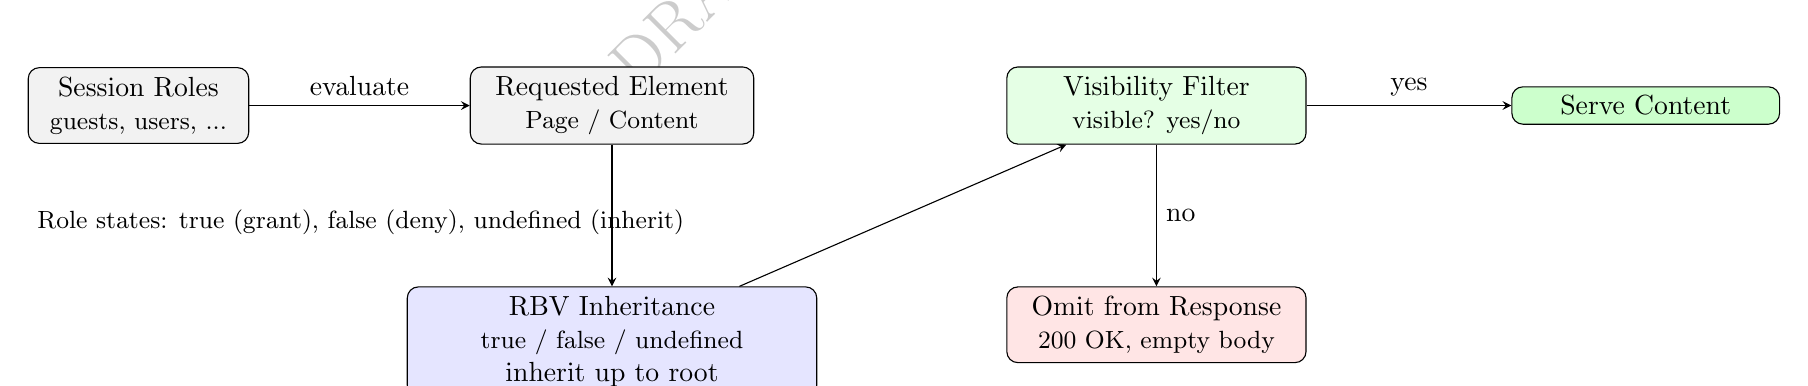
\begin{tikzpicture}[node distance=1.6cm,>=stealth,rounded corners,align=center]
	% Nodes
	\node[draw, fill=gray!10, minimum width=2.8cm] (roles) {Session Roles\\\small guests, users, ...};
	\node[draw, fill=gray!10, right=2.8cm of roles, minimum width=3.6cm] (element) {Requested Element\\\small Page / Content};
	\node[draw, fill=blue!10, below=1.8cm of element, minimum width=5.2cm] (inherit) {RBV Inheritance\\\small true / false / undefined\\inherit up to root};
	\node[draw, fill=green!10, right=3.2cm of element, minimum width=3.8cm] (filter) {Visibility Filter\\\small visible? yes/no};
	\node[draw, fill=green!20, right=2.6cm of filter, minimum width=3.4cm] (serve) {Serve Content};
	\node[draw, fill=red!10, below=1.8cm of filter, minimum width=3.8cm] (omit) {Omit from Response\\\small 200 OK, empty body};

	% Edges
	\draw[->] (roles) -- node[above] {evaluate} (element);
	\draw[->] (element) -- (inherit);
	\draw[->] (inherit) -- (filter);
	\draw[->] (filter) -- node[above] {yes} (serve);
	\draw[->] (filter) -- node[right] {no} (omit);

	% Legend
	\node[anchor=west] at ($(roles.south west)+(0,-1.0)$) {\small Role states: true (grant), false (deny), undefined (inherit)};
\end{tikzpicture}}%
\caption{Role-Based Visibility flow: roles are evaluated against element RBV with inheritance; invisible elements are omitted without error.}
\label{fig:rbv-flow}
\end{figure}

\paragraph{Role States}
Each role can be in one of three states:

\begin{description}
	\item[\texttt{true}] explicitly granted
	\item[\texttt{false}] explicitly denied
	\item[\texttt{undefined}] inherited from parent elements
\end{description}

Inheritance follows a recursive model from the content up to the site root.

\paragraph{Role Assignment}
Roles can be assigned to:
\begin{itemize}
	\item Individual contents
	\item Pages
	\item Areas
	\item Entire site
\end{itemize}
If no role is explicitly assigned, it inherits from its parent.

\paragraph{Default Role: Guests}
The \texttt{guests} role is automatically assigned to the portal home page and its contents. All other elements are invisible to guests unless explicitly made visible.

\subsection{Predefined Roles}

Spin the Web defines the following non-deletable roles:

\begin{itemize}
	\item \texttt{roots} \hfill\emph{superuser; see override below}
	\item \texttt{guests}
	\item \texttt{users}
	\item \texttt{administrators}
	\item \texttt{developers}
	\item \texttt{webmasters}
	\item \texttt{translators}
\end{itemize}

You may define additional roles as needed. A good starting point is your organizational chart.

\paragraph{Superuser override (\texttt{roots})}
The \texttt{roots} role represents a trusted superuser. When a session includes \texttt{roots}, the “no assignment found up to the site level” condition does \emph{not} cause a deny; instead, evaluation proceeds to the element’s \texttt{visible} flag. This does not change the semantics of \texttt{visible=false} (which still hides the element).

\subsection{RBV Decision Procedure}
\label{sec:rbv-decision}

With reference to Figure~\ref{fig:rbv-flow}, the Web Spinner applies Role-Based Visibility (RBV) using the following precise rules. Let \emph{roles} be the set of roles in the current session; visibility flags are tri-state \{\texttt{true}, \texttt{false}, unset\}, where unset is treated as \texttt{true}.

\paragraph{Page decision}
\begin{enumerate}
	\item If the requested page is the Home page, \textbf{ALLOW} by default.
	\item Else, if no authorization for any of the session roles is found on the page or any ancestor (page \textrightarrow{} area \textrightarrow{} site), \textbf{DENY} — \emph{unless} the session has the \texttt{roots} role, in which case continue to step 3.
	\item Else, if \texttt{page.visible} is \texttt{false}, \textbf{DENY} and \emph{navigate to the Home page}.
	\item Otherwise, \textbf{ALLOW}.
\end{enumerate}

\paragraph{Content decision (for each content on an allowed page)}
\begin{enumerate}
	\item If the content or its ancestors (page \textrightarrow{} area \textrightarrow{} site) define authorizations for the session roles:
		\begin{enumerate}
			\item If none of those authorizations evaluate to \texttt{true}, \textbf{DENY}.
			\item Else, if \texttt{content.visible} is \texttt{false}, \textbf{DENY}.
			\item Otherwise, \textbf{ALLOW}.
		\end{enumerate}
	\item If no role assignment for any session role is found all the way up to the site level, treat as an \emph{explicit deny} — \emph{unless} the session has the \texttt{roots} role, in which case evaluate \texttt{content.visible}: if \texttt{false} then \textbf{DENY}, otherwise \textbf{ALLOW}.
\end{enumerate}

\paragraph{Defaults and inheritance}
\begin{itemize}
		\item Pages are \emph{default-deny} (unless Home), requiring an explicit or inherited allow for at least one session role, and \texttt{visible} must not be \texttt{false}. If no role assignment is found all the way to the site level, treat the outcome as an \emph{explicit deny}; sessions with the \texttt{roots} role bypass this specific condition and proceed to the \texttt{visible} check.
		\item Contents without any role assignment up to the site level are \emph{explicitly denied}. Sessions with the \texttt{roots} role bypass only this condition and proceed to the \texttt{visible} check.
		\item RBV inherits up the hierarchy; evaluation short-circuits at the nearest level that defines role entries. If none are found by the time the site is reached, the result is an explicit deny (subject to the \texttt{roots} override above).
\end{itemize}

\section{User Session Management}
\label{sec:session-management}

The Web Spinner maintains stateful user sessions to manage authentication, authorization, and personalization:

\subsection{Session Establishment}

When a user first accesses the portal, a new session is created with a unique identifier; a guest user is set as the session user (assigned the \texttt{guests} role). Sessions are maintained using cookies, JWT tokens, or other mechanisms.

\subsection{Authentication Integration}

The system integrates with various authentication providers (LDAP, OAuth, SAML, etc.) to verify user credentials and establish their identity.

\subsection{Role Assignment}

Once authenticated, the user's roles are determined through integration with identity providers or internal role mappings. These roles are cached in the session for performance.

\subsection{Session State}

The session maintains:
\begin{itemize}
	\item User identity and roles
	\item Current language preference
	\item Navigation history
	\item Cached command results (when appropriate)
	\item Active datasource connections
\end{itemize}

\section{Request Routing and Processing}
\label{sec:request-routing}

The Web Spinner handles incoming HTTP requests through a sophisticated routing mechanism:

\subsection{URL Parsing}

Incoming URLs are parsed to extract the area/page/content hierarchy. For example:
\begin{itemize}
	\item \texttt{https://portal.acme.com/sales/dashboard} → Area: "sales", Page: "dashboard"
	\item \texttt{https://portal.acme.com/sales/dashboard/orders-table} → Area: "sales", Page: "dashboard", Content: "orders-table"
\end{itemize}

\subsection{Element Resolution}

Using the pre-built routing table, URLs are resolved to specific \wbdl{} elements. Runtime outcomes:
\begin{itemize}
	\item \textbf{Pages}: If the URL resolves to a page that is not visible to the current session (per Figure~\ref{fig:rbv-flow} and \secref{sec:rbv-decision}), the user is taken to the \textbf{Home page}. If the path itself is invalid, the nearest site or area main page is served.
	\item \textbf{Contents}: If a content is not visible, it is omitted entirely and the request returns \texttt{200 OK} with an empty body. If the path is invalid, no result is returned.
\end{itemize}

\subsection{Protocol Handling}

The Web Spinner supports both HTTP and WebSocket protocols:
\begin{description}
	\item[\textbf{HTTP}]: Used for standard page and content requests, following RESTful principles
	\item[\textbf{WebSocket}]: Used for real-time content updates, live data feeds, and interactive features
\end{description}

\section{Visibility and Authorization Engine}
\label{sec:authorization-engine}

Before any content is delivered, the Web Spinner performs comprehensive authorization checks. See \secref{sec:security} for the visibility model and predefined roles; this section focuses on runtime enforcement:

\subsection{Role-Based Filtering}

For each requested element (page or content), the visibility rules are evaluated against the user's session roles:
\begin{itemize}
	\item Elements with no matching role rules inherit visibility from their parent elements
	\item The hierarchical check continues up to the root element
	\item Elements without explicit or inherited visibility permissions are denied by default
\end{itemize}

\subsection{Dynamic Filtering}

Visibility checks are performed in real-time for every request, ensuring that changes to user roles or permissions take immediate effect.

\subsection{Secure Response Generation}

Only authorized elements are included in the response. Unauthorized elements are completely omitted, preventing information leakage.

\section{Content Request and Response Cycle}
\label{sec:content-cycle}

The Web Spinner handles content requests through a multi-stage process:

\subsection{Page Structure Delivery}

When a page is requested, the Web Spinner:
\begin{itemize}
	\item Identifies all visible \texttt{STWContent} elements for the page
	\item Returns a lightweight response containing the list of content slugs and their metadata
	\item Includes section assignments and sequencing information for layout
\end{itemize}

\subsection{Asynchronous Content Fetching}

The client then requests individual content elements:
\begin{itemize}
	\item Each content request triggers a separate web socket call to the Web Spinner
	\item Content elements are fetched in parallel, improving perceived performance
	\item Each content element is processed independently, allowing for granular caching and error handling
\end{itemize}

\subsection{Content Processing Pipeline}

For each content request, the Web Spinner:
\begin{enumerate}
	\item Validates user authorization for the specific content element
	\item Resolves the associated datasource and command
	\item Processes the command through the \wbpl{} (Webbase Placeholders Language) engine
	\item Executes the processed command against the datasource
	\item Applies the content layout transformation
	\item Returns the rendered content or raw data (depending on the request type)
\end{enumerate}

\section{Datasource Connection and Command Management}
\label{sec:datasource-management}

The Web Spinner maintains a sophisticated datasource management system:

\subsection{Connection Pooling}

Database and API connections are pooled and reused across requests to optimize performance and resource utilization.

\subsection{Command Processing}

Raw queries defined in \texttt{STWContent} elements undergo several processing steps:

\begin{description}
	\item[\textbf{\wbpl{} Processing}]: Placeholders are resolved using session data, URL parameters, and global variables
	\item[\textbf{Security Validation}]: Processed queries are validated to prevent injection attacks
	\item[\textbf{Optimization}]: Command plans may be cached for frequently-executed queries
\end{description}

\subsection{Multi-Datasource Support}

The system supports heterogeneous datasources:

\begin{description}
	\item[\textbf{Relational Databases}]: SQL queries with full \wbpl{} placeholder support
	\item[\textbf{\rest{} APIs}]: HTTP requests with parameter substitution and response transformation
	\item[\textbf{NoSQL Databases}]: Native command languages (MongoDB, Elasticsearch, etc.)
	\item[\textbf{File Systems}]: Direct file access and processing
\end{description}

\subsection{Error Handling}

Datasource errors are gracefully handled:
\begin{itemize}
	\item Connection failures trigger automatic retry logic
	\item Command errors are logged and appropriate error responses are returned
	\item Partial failures in multi-content pages don't affect other content elements
\end{itemize}

\section{Performance Optimization and Timeout Management}
\label{sec:performance-optimization}

The Web Spinner implements several performance and reliability features:

\subsection{Content Timeouts}

Each content element has configurable timeout settings:

\begin{description}
	\item[\textbf{Command Timeout}]: Maximum time allowed for datasource queries
	\item[\textbf{Layout Timeout}]: Maximum time for layout compilation and rendering
	\item[\textbf{Total Request Timeout}]: Overall timeout for content delivery
\end{description}

\subsection{Caching Mechanisms}

Multiple levels of caching improve performance:

\begin{description}
	\item[\textbf{Command Result Caching}]: Datasource results are cached based on command signatures
	\item[\textbf{Layout Caching}]: Compiled layouts are cached until templates change
	\item[\textbf{Response Caching}]: Complete HTTP responses may be cached for static content
\end{description}

\subsection{Load Balancing}

Multiple Web Spinner instances can operate in parallel:
\begin{itemize}
	\item Session affinity ensures consistent user experience
	\item Shared cache layers enable scaling across multiple servers
	\item Health monitoring ensures failed instances are automatically excluded
\end{itemize}

\subsection{Monitoring and Metrics}

The Web Spinner provides comprehensive monitoring:
\begin{itemize}
	\item Request/response times and throughput metrics
	\item Datasource performance and error rates
	\item User session analytics and behavior patterns
	\item System resource utilization and capacity planning data
\end{itemize}

This architecture ensures that the Web Spinner can handle enterprise-scale workloads while maintaining high performance, security, and reliability standards.

\section{Looking Forward}
\label{sec:webspinner-forward}

At this point, we have a powerful engine and a sophisticated set of languages. However, asking developers to write raw \wbdl{} in a text editor, manage resources via the command line, and test queries in a separate database tool would be laborious and inefficient. How can we streamline this development process?

This is where the \textbf{Spin the Web Studio} comes in. The Studio, itself a \webbaselet{}, provides a comprehensive, integrated development environment for building, testing, and deploying \webbase{s}. It is the testing ground for the entire Web Spinner ecosystem and an essential tool for any serious developer. The next chapter will be dedicated to exploring the Studio's rich feature set.

% Chapter: Spin the Web Studio
\chapter{Spin the Web Studio: An Integrated Development Environment}
\label{chap:studio}

\begin{quote}
\textit{"The best way to predict the future is to invent it."} \\
— Alan Kay
\end{quote}

\section{The Need for an Integrated Environment}
\label{sec:studio-need}

While the \wbdl{} and \wbpl{} languages provide a powerful declarative framework for defining enterprise portals, and the \webspinner{} engine offers a robust runtime, the development experience can still be laborious. Without a dedicated toolset, a developer would be forced to:

\begin{itemize}
    \item Write and edit complex \wbdl{} files in a standard text editor, without syntax highlighting, validation, or autocompletion.
    \item Manage portal resources, such as datasources and user roles, through command-line interfaces or direct database manipulation.
    \item Create and test \wbpl{} queries in a separate database management system, disconnected from the portal context.
    \item Manually compile and deploy the \webbase{} to see the results of any changes.
\end{itemize}

This fragmented workflow is inefficient, error-prone, and a significant barrier to productivity. To address these challenges, the \textbf{Spin the Web Studio} was created.

\section{Introducing the Spin the Web Studio}
\label{sec:studio-intro}

The Spin the Web Studio is a webbased development environment designed specifically for building, testing, and managing \webbase{s}. It streamlines the entire development lifecycle, from initial design to final deployment, providing a single, coherent interface for all development tasks.

Crucially, the Studio is not an external, standalone application. It is itself a \textbf{\webbaselet{}}, built using the very same technologies it helps to create. This has two profound implications:

\begin{enumerate}
    \item \textbf{The Ultimate Testing Ground}: The Studio serves as the primary testing ground for the \webspinner{} engine and the entire Spin the Web framework. Every feature of the framework must be robust and performant enough to run the Studio itself.
    \item \textbf{Part of the Virtualized Portal}: As a \webbaselet{}, the Studio can be seamlessly integrated into any \webbase{}. This allows developers with the appropriate permissions to access the development environment directly from within the live portal, making it a true part of the virtualized web portal.
\end{enumerate}

\section{Studio Architecture and Activation}
\label{sec:studio-architecture}

The Studio operates as a specialized \webbaselet{} that is added to the portal \webbase{} and is accessible to users with developer permissions when they log in. The studio remains hidden until activated by the developer using the keyboard shortcut \textbf{Alt+F12}.

Upon activation, the Studio transforms the portal interface into a full-featured development environment with the following key components:

\begin{description}
    \item[Action Bar] Provides quick access to the Studio functions.
    \item[Side Bar] Houses multiple views including interactive \webbase{} hierarchy, portal folder contents, search capabilities, debugging tools, source control integration, and Studio settings.
    \item[Status Bar] Displays development status information, compilation results, and system feedback.
    \item[Panel] Contains additional development tools, terminal access, and debugging output.
    \item[Main Section] Features a tabbed interface where the live portal is displayed in a persistent browser tab alongside other editors.
\end{description}

\subsection{Unique Browser Tab Integration}
\label{sec:studio-browser-tab}

One of the Studio's most innovative features is its tab management system. The main section displays the live portal in a special browser tab that cannot be closed, ensuring developers always maintain visual connection to their running application. Portal resources such as files, configurations, and logs can be opened in separate tabs for editing and review.

This design creates an in-place development experience where:
\begin{itemize}
    \item Changes to \wbdl{} files are immediately reflected in the persistent portal view
    \item Developers can interact with the live portal while simultaneously editing its underlying code
    \item The development environment becomes part of the portal ecosystem rather than an external tool
\end{itemize}

\subsection{Side Bar Navigation}
\label{sec:studio-sidebar}

The Studio's side bar provides comprehensive navigation and development tools through multiple specialized views:

\begin{description}
    \item[Interactive \webbase{} Hierarchy] A tree view displaying the complete structure of the \webbase{}, allowing developers to navigate between \webbaselets{}, datasources, and configurations with visual context.
    \item[Portal Primary Folder Contents] Direct access to the portal's file system, enabling quick file management and resource organization.
    \item[Search] Comprehensive search capabilities across both \webbase{} definitions and folder contents, supporting pattern matching and content searches.
    \item[Debugging] Integrated debugging tools for \wbpl{} queries, \webbaselet{} execution, and runtime diagnostics.
    \item[Source Control] Built-in version control integration for tracking changes to \webbase{} definitions and portal resources.
    \item[Studio Settings] Customization options for the development environment, including themes, editor preferences, and workflow configurations.
\end{description}

\section{Key Features of the Studio}
\label{sec:studio-features}

The Studio is organized into several key modules, each addressing a specific aspect of \webbase{} development.

\subsection{The WBDL Editor}
A rich text editor with full support for the \wbdl{} syntax, featuring:
\begin{itemize}
    \item Syntax highlighting for improved readability.
    \item Real-time validation to catch errors as you type.
    \item Autocompletion for element names and properties.
    \item A hierarchical tree view for easy navigation of the \webbase{} structure.
\end{itemize}

\subsection{The WBPL Command Builder}
An interactive tool for creating, testing, and debugging \wbpl{} queries:
\begin{itemize}
    \item A graphical interface for building complex queries.
    \item The ability to execute queries against live datasources and view the results instantly.
    \item A "persona simulator" to test queries under different user roles and contexts.
\end{itemize}

\subsection{Resource Management}
A centralized dashboard for managing all portal resources:
\begin{itemize}
    \item \textbf{Datasource Configuration}: Connect to and manage various data sources (databases, APIs, etc.).
    \item \textbf{User and Role Management}: Define user roles and assign permissions.
    \item \textbf{Asset Library}: Upload and manage static assets like images, CSS, and JavaScript files.
\end{itemize}

\subsection{Live Preview and Deployment}
The Studio provides a real-time preview of the portal as you build it. Developers can instantly see how their changes will look and behave. When development is complete, the Studio offers one-click deployment to staging or production environments.

\section{Looking Forward}
\label{sec:studio-forward}

The Spin the Web Studio completes the conceptual picture of the framework, providing the "workshop" necessary to build with the "blueprint" and the "engine." It transforms \webbase{} development from a manual, error-prone task into a streamlined, interactive experience.

Now that we have covered the complete set of tools in the framework—from the declarative languages to the runtime engine and the IDE—the next chapter will ground these concepts in reality. We will examine the specific technology stack and implementation details of the reference Web Spinner, revealing how these architectural principles are translated into running code.

% Chapter 11: Technology Stack and Implementation
\chapter{Technology Stack and Implementation}
\label{chap:technology}

This chapter documents the concrete technologies used to implement the web spinner mechanics and how the theoretical constructs from Part II are realized in a working system.

\section{Runtime and Languages}
The reference implementation is written in TypeScript and runs on the Deno runtime:
\begin{itemize}
	\item Deno runtime and TypeScript for server-side logic
	\item Standard Web APIs (URL, URLSearchParams, Fetch, Crypto) leveraged directly in server code
	\item No Node.js dependency; tasks and scripts are run via Deno (e.g., CSS/JS minification)
	\item Containerization via a multi-stage Dockerfile based on denoland/deno:alpine
\end{itemize}

\subsection{Why Deno for the \webspinner?}
Choosing Deno aligns the engine with the platform’s web-first design and keeps the implementation close to the browser runtime:
\begin{itemize}
	\item \textbf{TypeScript end-to-end:} one language for the spinner, utilities, and any shared logic with client code.
	\item \textbf{Web APIs in the server:} standard \texttt{URL}, \texttt{Request/Response}, \texttt{Fetch}, and \texttt{Crypto} lower cognitive load and reduce bespoke abstractions.
	\item \textbf{Secure-by-default:} explicit permissions (fs, net, env) encourage disciplined deployment.
	\item \textbf{Batteries included:} built-in formatter, test runner, task runner, and linting simplify tooling.
	\item \textbf{Simple deploys:} reproducible Docker images and a single binary runtime keep operations light.
	\item \textbf{ESM-first:} native modules and top-level \texttt{await} fit the compilation model used by \wbll and \wbpl tooling.
\end{itemize}

Other implementations are welcomed, provided they adhere to the specifications and interoperability guidelines set forth by the \organization{}.

\section{High-Level Architecture}
The spinner is a server that understands WBDL. On each request it:\footnote{See also the ``Paradigm'' section in the implementation README}
\begin{enumerate}
	\item Establishes or resumes a session (user, roles, locale, placeholders)
	\item Ensures the requested WBDL/Webbase is loaded into an in-memory tree
	\item Decides whether to respond with a resource directly or with a list of REST calls the client should make (async via WebSockets)
	\item Renders contents on demand using WBLL-driven layouts and returns HTML fragments/resources
\end{enumerate}

\section{Core Elements and Site Tree}
The in-memory model mirrors the WBDL structure:
\begin{itemize}
	\item \textbf{STWSite} (singleton root), \textbf{STWArea}, \textbf{STWPage}, \textbf{STWContent}
	\item All derive from an abstract \textbf{STWElement} providing identity, naming, localization, hierarchy, and export to WBDL
	\item A content type (e.g., Text, Table, Menus, Breadcrumbs, Calendar, Code Editor, ...), implemented under \texttt{stwContents/}, encapsulates data access and rendering concerns
\end{itemize}

\section{Rendering Pipeline: WBLL and WBPL}
Presentation is described with WBLL (Webbase Layout Language), interpreted by a layout engine:
\begin{itemize}
	\item WBLL strings are tokenized and validated; tokens drive generation of a specialized render function
	\item Token handlers cover inputs, lists, links, media, buttons/actions, and structural fragments; they build HTML using placeholders and field values
	\item WBPL expressions provide string interpolation and conditional/functional logic within layouts and settings
	\item Placeholders (e.g., \verb|@@name|) merge session, request, and record values
\end{itemize}

\section{Request Flow in Practice}
For a content render request:
\begin{enumerate}
	\item The session determines visibility (role-based) and language
	\item The content locates its WBLL layout for the current language
	\item Records are fetched (via a datasource or parameters); the first row and fields hydrate placeholders
	\item The compiled WBLL render function executes, producing the HTML body; optional header/footer wrappers apply
\end{enumerate}

\section{Security, Localization, and State}
\begin{itemize}
	\item \textbf{Visibility}: role-based flags inherited along the element tree control exposure of nodes
	\item \textbf{Localization}: localized properties (names, slugs, messages) are resolved through the session
	\item \textbf{State}: per-session placeholders and content-level settings influence rendering and actions
\end{itemize}

\section{Build, Tooling, and Deployment}
\begin{itemize}
	\item Deno tasks: merge and minify static assets (e.g., CSS merger, JS minifier) for the \texttt{public/} client assets
	\item Tests: parsing and evaluation tests for WBPL ensure correctness of expressions and escaping
	\item Docker: multi-stage build caches Deno dependencies and ships a non-root runtime image
\end{itemize}

\section{Where the Mechanics Live (Guide to Source)}
The following folders in the reference implementation contain the mechanics described above:
\begin{itemize}
	\item \texttt{stwElements/}: \textit{STWElement}, \textit{STWSite}, \textit{STWArea}, \textit{STWPage}, \textit{STWContent}
	\item \texttt{stwContents/}: concrete contents and \textit{WBLL} engine (layout parsing/rendering)
	\item \texttt{tests/}: WBPL and layout-related unit tests
	\item \texttt{public/}: client-side scripts, styles, and SPA shell
	\item \texttt{tasks/}: Deno-powered dev/build utilities (e.g., minification, CSS merge)
\end{itemize}

\section{Example: From WBDL to HTML}
At a glance:
\begin{enumerate}
	\item WBDL defines the site tree; the spinner builds an in-memory model at startup/load
	\item A user navigates to a page; the spinner locates the route and the associated contents
	\item Each content loads data (if needed), prepares placeholders, and renders its WBLL layout
	\item The server responds with an HTML fragment or instructs the client to fetch multiple fragments via REST/WebSockets
\end{enumerate}

\noindent This chapter has bridged theory and implementation, showing how the abstract mechanics of the Web Spinner are realized in a modern technology stack. With the platform's construction now fully detailed—from its languages to its engine and development tools—our focus shifts from building the framework to using it.

The next part of this book begins the practical guide for developers, covering the development models and methodologies for designing and building effective web portals with the platform we have just described.


% Part III: The Portal
\part{The Portal}
% Part III: The Portal

\chapter*{Introduction to Part III: The Portal}
\addcontentsline{toc}{chapter}{Introduction to Part III: The Portal}
\label{part:implementation}

\begin{quote}
\textit{"Structure is not just a means to a solution. It is the solution."} \\
— Alexandra V. Agranovsky
\end{quote}

With the Spin the Web framework fully specified in Part II, this part transitions from engineering blueprints to practical application. It serves as the developer's guide to the models and methodologies for *using* the framework to design, build, and structure a real-world enterprise portal.

This part now divides implementation into two complementary dimensions:
\begin{itemize}
	\item \textbf{Portal Contents (Structure, Semantics, Information)} — Modeling Areas, Pages, and Content blocks; embedding documentation; designing navigation, search, and task-oriented information architecture (\cref{chap:portal-contents}).
	\item \textbf{Portal Visuals (Presentation, Layout, Interaction)} — Translating structure into accessible, brand-aligned, performant user interfaces while preserving semantic integrity (\cref{chap:portal-visuals}).
\end{itemize}

Throughout, we reference the public website \href{https://spintheweb.org}{spintheweb.org} and the companion \studio{}—both built with the framework—as running examples of the patterns described here. For an overview of the community catalog used to discover and rate webbaselets, see the Ecosystem webbaselet in \cref{sec:app-ecosystem}.

By the end of this part, you will have a clear methodology for designing and building sophisticated web portals using the Spin the Web framework—treating structure and presentation as orthogonal layers that evolve independently yet harmonize in the delivered experience.

% Chapter: Implementing Portal Contents
\chapter{Implementing Portal Contents: Structure, Semantics, and Information Flow}
\label{chap:portal-contents}

\begin{quote}
\textit{"Structure is the substrate of meaning; when well designed it becomes self-documenting and accelerates delivery."}
\end{quote}

This chapter covers how to model and implement the *informational side* of an enterprise portal using \wbdl{}: Areas, Pages, and Content blocks as semantic anchors; embedded documentation as a living knowledge system; and patterns for navigation, search, and task execution. The emphasis is on how structure transforms raw enterprise data into durable, navigable knowledge assets.

% Placeholder sections to be populated by extracted/adapted material
\section{From Organization to Information Architecture}
\label{sec:contents-org-to-ia}
The starting point for portal content modeling is the enterprise itself. Business functions, departments, service domains, and stakeholder-facing capabilities provide the *semantic inventory* that becomes your top-level \texttt{STWArea} set. Mapping is a translation exercise:
\begin{enumerate}
	\item Collect the official organizational chart(s) and cross-functional process maps.
	\item Identify external-facing vs. internal-only domains; decide which are public, private, or hybrid.
	\item Normalize naming (short, role-recognizable labels) and prune redundancies.
	\item Annotate each candidate Area with primary audiences, core data domains, and governing policies.
	\item Prioritize rollout sequence (critical operations first, supporting domains next, exploratory later).
\end{enumerate}
\paragraph{Example Top-Level Areas} A manufacturing enterprise might define: Sales, Administration, Backoffice, Technical Office, Products \& Services. Each becomes an \texttt{STWArea} root for subordinate Pages and Content.

Area definitions embed *living documentation* through localized \texttt{name}, \texttt{description}, and \texttt{keywords}. This collapses the distance between operational knowledge and runtime structure: the portal itself becomes the manual.

\section{Hierarchical Semantics and Namespaces}
Hierarchy provides cognitive compression. The \emph{Hierarchical Namespace Pattern} organizes content so users predict where information lives. Recommended principles:
\begin{itemize}
	\item Depth over width only when each level adds semantic clarity.
	\item Keep sibling counts manageable (7\,$\pm$\,2 heuristic for primary navigation tiers).
	\item Use stable identifiers (slugs) for Areas/Pages to preserve deep links and audit trails.
	\item Reflect role segmentation (what differs by role) at the \texttt{STWContent} or conditional rendering layer rather than duplicating structural nodes.
\end{itemize}
Roles shape *visibility* and *interaction surfaces* but should not fork the structural namespace unnecessarily. This separation sustains maintainability and consistent analytics.

\section{Documentation Through Structure}
Every \wbdl{} element (Site, Area, Page, Content) hosts localized \texttt{description} and \texttt{keywords}. These fields form a vertically integrated documentation system that can encode: quality policies, compliance references, process identifiers, KPIs, audit obligations, data classification tags, and internal taxonomy terms. \autoref{tab:doc-scope} summarizes scope alignment.

\begin{description}
	\item[Site] Mission, global quality policy, enterprise standards.
	\item[Area] Departmental procedures, regulatory scope, operating KPIs.
	\item[Page] Process walkthroughs, workflow prerequisites, exception handling.
	\item[Content] Field-level rules, validation, data retention, privacy notes.
\end{description}

Embedding this metadata enables: contextual help, machine-assisted authoring, internal semantic search, automated compliance extraction, and AI augmentation (linking processes to data touchpoints).

\begin{table}[h]
	\centering
	\caption{Documentation scope by structural level}\label{tab:doc-scope}
	\begin{tabularx}{\textwidth}{l l X X}
		\toprule
		\textbf{Level} & \textbf{Primary Focus} & \textbf{Typical Metadata} & \textbf{Example Questions Enabled} \\
		\midrule
		Site & Enterprise Mission & Mission, quality policy, audit standards, global KPIs & What is the overarching mission? Which global standards govern all Areas? \\
		Area & Department / Domain & Procedures, regulatory scope, data domains, risk class & Which regulations apply to this domain? Who owns the process? \\
		Page & Process / Journey & Workflow steps, prerequisites, exception handling, SLA & What happens before/after this step? What are escalation paths? \\
		Content & Field / Action Unit & Validation rules, retention, privacy flags, policy codes & Can this value be exported? How long is data retained? \\
		\bottomrule
	\end{tabularx}
	\vspace{0.5em}
	\footnotesize The metadata lattice supports contextual help, semantic search ranking, compliance extraction, and AI-assisted authoring.
\end{table}

\section{Core Page Archetypes}
Across domains three archetypes dominate main content regions:
\begin{itemize}
	\item \textbf{Dashboards}: Multi-source summaries for situational awareness and prioritization. Favor glanceable KPIs, deltas, and exception surfacing.
	\item \textbf{Tabular / List Views}: Filterable, paginated, sometimes hierarchical or pivot-capable collections enabling search+select workflows.
	\item \textbf{Detail Views}: Focused inspection/editing surfaces for a single entity with contextual navigation (previous/next, related entities, timeline overlays).
\end{itemize}
Composite pages combine archetypes (e.g., miniature dashboard widgets above a list). Resist uncontrolled aggregation—each archetype should answer a distinct question.

\section{User Journeys and Page Design}
Pages (\texttt{STWPage}) embody discrete user tasks or journeys. Design methodology:
\begin{enumerate}
	\item \textbf{Task Enumeration}: Elicit core user goals per Area (create quote, approve order, analyze defect rate).
	\item \textbf{Journey Mapping}: Sequence states and data intersections; identify required contextual jumps (entity cross-links) to minimize session fragmentation.
	\item \textbf{Structural Allocation}: Assign each journey to a Page; merge only if cognitive load stays low and authorization scopes match.
	\item \textbf{Section Layout}: Header (global actions), sidebars (navigation, filters, summaries), main body (primary archetype), footer (feedback, contacts).
	\item \textbf{Instrumentation}: Embed identifiers and metadata for analytics, ticketing, and performance tracing.
\end{enumerate}
\paragraph{Integrated Ticketing} A mature portal treats structure itself as a support surface. Ticket submissions should auto-capture structural scope (site/area/page/content IDs), user locale, and active filters. This converts qualitative feedback into structured, triage-ready data.

\section{Building with Content Blocks}
\texttt{STWContent} instances are atomic functional or informational units: forms, tables, charts, grids, banners, maps, metrics, documents. Composition principles:
\begin{itemize}
	\item \textbf{Single Responsibility}: Each block answers one primary question or supports one action cluster.
	\item \textbf{Declarative Data Binding}: Use \wbpl{} for parameterized queries; keep transformation logic close to data retrieval for transparency.
	\item \textbf{Progressive Disclosure}: Lazy-load heavy or low-priority content blocks to reduce initial cognitive and performance load.
	\item \textbf{Embedded Governance}: Include validation rules, policy codes, and retention hints inside \texttt{description} metadata.
	\item \textbf{Reusability}: Parameterize commonly repeated patterns (e.g., entity summary panels) rather than cloning definitions.
\end{itemize}
\paragraph{Example Composition} A public "Products" page may combine: hero banner (static), category menu (dynamic list), product grid (dynamic, filtered), featured carousel (dynamic curated), and call-to-action block—each a discrete \texttt{STWContent}.

\section{Search, Discovery, and Internal SEO}
Localized \texttt{keywords} and \texttt{description} fields drive internal search relevance. Two complementary modes:
\begin{description}
	\item[Global Search] Traverses full structural graph; returns heterogenous results ranked by metadata quality, usage signals, and recency.
	\item[In-Context Search] Operates within the active Page scope: filters list/table rows, quick-finds form fields, queries localized help.
\end{description}
Design guidance: persistent global search affordance (often header); proximal in-context search control near target content. Provide keyboard shortcuts, accessible labeling, and query history. Treat internal search analytics as a requirements radar (unmet search intent indicates structural or content gaps).

\section{Patterns and Evolution}
Long-term iteration reveals recurring cycles: pattern recognition $\rightarrow$ insight $\rightarrow$ abstraction $\rightarrow$ simplification. Content modeling matures by:
\begin{itemize}
	\item Consolidating duplicated structures into parameterized definitions.
	\item Elevating cross-cutting concerns (authorization tags, retention policies) into shared vocabularies.
	\item Refactoring deep hierarchies when navigation analytics show friction.
	\item Capturing emergent naming conventions to stabilize taxonomy.
	\item Instrumenting evolution (version history of structural nodes) to support audits and AI summarization.
\end{itemize}
The endpoint is elegant simplicity: a minimal, expressive structure that scales without combinatorial explosion.

\section{Conclusion}
The content layer transforms disparate enterprise data into structured, navigable, contextual information assets. By treating every node (Area/Page/Content) as both functional unit and documentation carrier, the portal becomes a continuously evolving, queryable knowledge base that supports operations, compliance, and learning.

% Chapter: Implementing Portal Visuals
\chapter{Implementing Portal Visuals: Presentation, Layout, and Interaction}
\label{chap:portal-visuals}

\begin{quote}
\textit{"Visual design should disappear into function, letting users feel the system rather than notice it."}
\end{quote}

This chapter focuses on the *visual and interaction layer* of a Spin the Web portal: translating semantic structure into perceivable, accessible, performant, and brand-aligned experiences—without compromising the stability of information architecture defined in \cref{chap:portal-contents}. The goal is to make presentation an *orthogonal dimension*: evolvable, themable, and testable in isolation.

\section{Separation of Structure and Presentation}
Structure lives in \wbdl{}: Areas, Pages, and Content blocks define semantics, navigation graph, and documentation. Presentation lives in a theming and layout layer (CSS variables, design tokens, component library primitives) that consumes structural metadata. This separation yields:
\begin{itemize}
	\item \textbf{Predictable Evolution}: New visual themes deploy without structural migrations.
	\item \textbf{Stable Deep Links}: URLs and identifiers remain constant across redesigns.
	\item \textbf{Semantic Integrity}: Search, analytics, and AI augmentations operate on durable structure, not brittle selectors.
	\item \textbf{Test Focus}: Functional tests target structure and logic; visual regression suites target presentation surfaces.
\end{itemize}
Anti-patterns: encoding layout meaning into identifiers; duplicating Pages solely for cosmetic variants; baking brand colors into content definitions.

\paragraph{Design Tokens} Use an invariant token vocabulary (e.g., \texttt{color.surface.raised}, \texttt{space.xs}, \texttt{font.heading.scale}) mapped to concrete theme values. Tokens enable multi-brand deployments and dark/light adaptation with minimal churn.

\section{Layout Regions and Responsiveness}
Canonical regions: Header (global nav, identity, search), Primary Navigation (lateral or horizontal), Context Pane (filters, related entities), Main Content, Ancillary Panels (notifications, collaboration), Footer (legal, contact). Responsive strategy principles:
\begin{enumerate}
	\item \textbf{Mobile First Density}: Collapse non-critical side regions into overlay drawers; preserve primary task path above decorative brand elements.
	\item \textbf{Breakpoint Semantics}: Define breakpoints where interaction model changes (hover removed < tablet, multi-column grids collapse).
	\item \textbf{Progressive Disclosure}: Defer rendering of off-screen heavy panels until first invocation.
	\item \textbf{Adaptive, Not Just Responsive}: Personalize ordering of blocks based on role usage analytics while retaining structural IDs.
\end{enumerate}
Use CSS grid/flex abstractions aligned to tokenized spacing; avoid ad hoc pixel constants.

\section{Navigation Systems and Flow}
Navigation manifests user mental models of the structure. Layers:
\begin{description}
	\item[Global Navigation] Exposes top-level Areas; must be stable, sparse, and keyboard navigable.
	\item[Local Navigation] Contextual to an Area or Page section (tab sets, side menus) for lateral moves.
	\item[Breadcrumbs] Encode path memory; avoid redundancy when global navigation already fully mirrors hierarchy depth 1.
	\item[Inline Relational Links] Provide graph exploration (related entities, recent activity) without forcing full context switch.
\end{description}
Design heuristics: prefer \textit{predictable repetition} (consistent placement) over novelty; minimize hover-only affordances; provide explicit focus order. Instrument navigation events to surface friction (abandoned path segments, loop behaviors).

\paragraph{Image and Iconographic Navigation}\label{sec:image-nav}
Navigation can also be accomplished through \textbf{clickable images}, floor-plan style ``planimetries'', diagrams, or semantically meaningful icons. These affordances are powerful for spatial, facilities, product catalog, or process topology exploration. To integrate them without sacrificing accessibility or scalability:
\begin{itemize}
	\item \textbf{Semantic Redundancy}: Every image-driven affordance must have a parallel text link or ARIA-labelled control to support screen readers and search indexing.
	\item \textbf{Vector Over Raster}: Prefer SVG with distinct, focusable regions (using \texttt{<a>} or \texttt{role="link"}) instead of image maps on raster graphics; enables theming and high-DPI crispness.
	\item \textbf{Descriptive Tooltips}: Provide concise tooltips / \texttt{title} attributes; avoid encoding primary meaning solely in color or pictogram shape.
	\item \textbf{Responsive Hit Targets}: Ensure minimum target size (44\,px CSS) across breakpoints; adapt layout so targets do not cluster too densely on touch devices.
	\item \textbf{Keyboard Pathways}: Maintain logical tab order across hotspot regions; allow arrow-key or WASD navigation for spatial grids where appropriate.
	\item \textbf{Progressive Enhancement}: Initial load should render a textual list fallback while SVG/hotspot script enhancements hydrate.
	\item \textbf{Performance Budget}: Large planimetric diagrams should be chunked or lazily loaded; defer non-visible layers (e.g., annotations) until interaction.
	\item \textbf{Analytics Instrumentation}: Tag each hotspot with structural IDs (Area/Page/Content) and business semantics to measure navigation efficacy and dead zones.
	\item \textbf{Scalability}: For dynamic catalogs, auto-generate hotspot layers from the \wbdl{} structure rather than manually editing coordinates.
	\item \textbf{Theming}: Bind fills, strokes, and hover states to design tokens (not hard-coded colors) for dark mode and brand adaptations.
\end{itemize}
Use image-based navigation to \emph{accelerate discovery}, not to replace canonical hierarchical paths. Spatial or iconographic maps become a complementary entry surface feeding into the same stable URL and breadcrumb system.

\section{Dashboards, Tables, and Details}
Visual treatments align to archetype intent:
\begin{itemize}
	\item \textbf{Dashboards}: Prioritize contrast, succinct labeling, and anomaly highlighting. Limit cardinality of primary KPI tiles (7\,$\pm$\,2). Provide consistent tile grammar: label, value, delta, trend.
	\item \textbf{Tables / Lists}: Support density toggles (comfortable/compact), sticky headers, column personalization. Emphasize scannability: left-align textual identifiers, right-align numeric aggregates, reserve iconography for actionable states.
	\item \textbf{Detail Views}: Anchor with an identity bar (title, status, primary actions). Segment content with visual rhythm (spacing tiers) not heavy borders. Provide contextual next/previous navigation when part of a result set.
\end{itemize}
Cross-cutting: embed loading placeholders shaped like final content (skeletons) to reduce perceived latency; ensure empty states teach next action.

\section{Role-Based Visual Adaptation}
Authorization governs data visibility; visual adaptation communicates scope without fragmenting structure. Techniques:
\begin{itemize}
	\item Conditional display of Content blocks (retain layout placeholders to avoid jumpy reflow when possible).
	\item Progressive disclosure of advanced filters and bulk actions only for privileged roles.
	\item Declarative role tags bound to CSS utility classes for subtle emphasis (e.g., manager-only highlights).
	\item Unified audit overlay mode (toggle) to display why elements are hidden (for debugging and governance).
\end{itemize}
Avoid: duplicating Pages per role; mixing security logic into visual components instead of central policy engines.

\section{Feedback, Ticketing, and Observability}
Integrate a frictionless feedback loop aligned with structure (see \cref{chap:portal-contents} on instrumentation). Key UI constructs:
\begin{itemize}
	\item Inline issue trigger (icon/button) scoped to Page or Content block; auto-captures structural IDs, user locale, and viewport size.
	\item Session timeline panel exposing recent navigation, feature flags, and performance spans for support replication.
	\item Visual state indicators: latency spinners, deferred load badges, stale data warnings with last refresh timestamp.
	\item Observability overlay (admin only) highlighting render cost hotspots / API latency zones.
\end{itemize}
Close the loop: a ticket success toast with deep link to status; encourage user re-engagement instead of dead-end submission pages.

\section{Search Experience Design}
Two surfaces (global, in-context) must \textit{feel} unified. Global search: omnipresent field or icon opening a command palette style modal; supports keyboard invocation, fuzzy matching, and result type grouping. In-context search: embedded within tables, forms, or navigation panels, scoping results to current structural node.
\paragraph{Design Principles}
\begin{itemize}
	\item Immediate focus when opening global search; preserve prior query history with non-intrusive ghost text.
	\item Provide semantic filters (Area/Page) as chips; avoid forcing users to learn query DSL initially.
	\item Highlight matched substrings for learnable relevance model feedback.
	\item Offer keyboard preview navigation with real-time detail pane (no full navigation until commit).
\end{itemize}
Accessibility: ARIA roles (combobox, listbox), announce result counts, maintain logical tab order returning user to invoking control when dismissed.

\section{Accessibility and Inclusive Design}
Inclusive design is multiplicative: it improves efficiency for all users while enabling access for those with specific needs. Core practices:
\begin{itemize}
	\item Semantic HTML foundation; avoid \texttt{div}-only components.
	\item Color contrast meeting WCAG 2.1 AA (4.5:1 text, 3:1 large); test dark/light parity.
	\item Full keyboard operability: visible focus, logical order, skip links for main content.
	\item Motion reduction honoring prefers-reduced-motion; substitute subtle fades for large parallax.
	\item Localization readiness: mirrored layouts for RTL, flexible space for longer strings, numeric/date formatting.
	\item Assistive hints in metadata (descriptions) powering contextual help and screen reader summaries.
\end{itemize}
Adopt automated accessibility testing plus manual audits (screen reader smoke tests) in CI.

\section{Branding and Themability}
Brand expression emerges from typography scale, color system, shape language (radius, stroke), and motion curve palette. Implementation strategy:
\begin{enumerate}
	\item Define neutral base theme (grayscale, spacing, layout primitives).
	\item Layer brand-specific tokens (color, typography, motion) referencing base tokens—no hard-coded hex in components.
	\item Provide runtime theme switch (light/dark/high-contrast) with persisted user preference.
	\item Guard legibility: run contrast validation when updating token sets; reject failing combinations.
	\item Expose a Theme Inspector webbaselet for administrators to preview token diffs live.
\end{enumerate}
Multi-brand portals map different token sets to identical \wbdl{} structures, enabling re-use of governance and search analytics.

\section{Performance and Perceived Speed}
User perception hinges on \textit{time to meaningful interaction}. Strategies:
\begin{description}
	\item[Skeleton Screens] Mirror final layout; avoid generic spinners that reset user mental model.
	\item[Incremental Data Hydration] Stream primary entities first; defer secondary panels (analytics, recommendations).
	\item[Optimistic UI] Reflect user intent immediately (button state, provisional row) with reconcile fallback if server rejects.
	\item[Edge Caching] Cache static assets and token manifests at CDN; version tokens for instant theme rollbacks.
	\item[Resource Budgeting] Define performance budgets (kb per route, API latency SLOs) and surface violations in build pipeline.
\end{description}
Instrument Web Vitals (LCP, INP, CLS) and map to structural IDs for precise remediation. Performance data should be browsable through an internal observability webbaselet.

\section{Conclusion}
A disciplined visual layer preserves semantic clarity while amplifying usability, trust, and brand presence. By keeping presentation orthogonal to structure, portals remain evolvable: new themes, devices, and interaction models can emerge without refactoring the underlying \wbdl{} definitions. Visual excellence compounds: accessible, performant, token-driven interfaces reduce cognitive load and accelerate enterprise adoption.


% Part IV: The Roadmap
\part{The Roadmap}
% Part IV: The Future

\chapter*{Introduction to Part IV}
\addcontentsline{toc}{chapter}{Introduction to Part IV}
\label{part:roadmap}

This part looks ahead: emerging patterns, research directions, and opportunities for the Spin the Web ecosystem. It consolidates lessons from earlier parts and projects them into near- and long-term roadmaps.

Areas of exploration include interoperability with evolving web standards and APIs, performance and cost at scale, formal methods for validating specifications and transformations, and community-driven extension mechanisms.

\textit{A living roadmap.} This book is a continuous work in progress. Part IV serves as a staging area for forward-looking ideas and experiments. As proposals mature and are implemented, they are promoted to:
\begin{itemize}
  \item Part II (The Framework) --- when they affect the framework’s languages, runtime, or tooling.
  \item Part III (The Web Portal) --- when they shape methods, patterns, or models for portal design and delivery.
\end{itemize}

\noindent The chapter that follows, \emph{The Roadmap} (\cref{chap:roadmap}), collects the most promising threads and defines criteria for promotion into the main body of


% Chapter 14: The Roadmap

\chapter{The Roadmap}
\label{chap:roadmap}

This chapter explores the transformative potential of Spin the Web as it evolves beyond individual portal development toward intelligent, interconnected business ecosystems. We examine how AI agents can enhance portal functionality while envisioning a future where structured corporate portals enable seamless machine-to-machine communication across global business networks.

\section{Agentic UX}
\begin{itemize}
	\item Contextual copilots embedded within areas/pages
	\item Task-oriented flows that orchestrate multiple contents and APIs
	\item Natural-language prompts mapped to parameterized actions
\end{itemize}

\section{Knowledge and Reasoning}
\begin{itemize}
	\item Retrieval pipelines grounded in the webbase, logs, and domain docs
	\item Guardrails and policy evaluation layered over actions
	\item Transparent, auditable traces for enterprise adoption
\end{itemize}

\section{Learning Loops}
\begin{itemize}
	\item Implicit feedback from usage, explicit ratings for outcomes
	\item Continuous improvement of layouts, queries, and flows
	\item Safe experimentation with feature flags and A/B variants
\end{itemize}

\section{Operational Model}
\begin{itemize}
	\item Private inference endpoints and on-prem models for compliance
	\item Event streams for real-time adaptations and monitoring
	\item Cost controls, quotas, and quality-of-service tiers
\end{itemize}

\section{Standards and Interop}
\begin{itemize}
	\item Schema-first contracts for tools and agent actions
	\item Portable traces and evaluation datasets
	\item Alignment with emerging agent frameworks and security best practices
\end{itemize}

\section{The Digital Ecosystem Vision: Machine-to-Machine Business Communication}
\label{sec:digital-ecosystem-vision}

Envision a digital world where every company maintains a structured web portal built on declarative principles—a world where business communication transcends human interfaces to enable seamless machine-to-machine interaction. In this ecosystem, corporate portals would serve as standardized digital representations of organizations, with each portal exposing structured data through consistent \wbdl{} definitions that machines can interpret and interact with automatically.

Consider the transformative potential: when suppliers, customers, partners, and service providers all maintain portals with standardized structures, business processes could become truly automated. A manufacturing company's portal could automatically command supplier portals for inventory levels, pricing updates, and delivery schedules. Customer portals could seamlessly integrate with vendor systems for real-time order tracking, automated reordering, and predictive maintenance scheduling. Regulatory compliance could be achieved through automated data exchange between corporate portals and government systems.

This vision extends the concept of eBranding into eMachineReading—where organizations design their digital presence not only for human stakeholders but also for automated business processes. The hierarchical documentation principles embedded within \wbdl{} structures would provide the semantic foundation necessary for machines to understand business context, process flows, and data relationships. Quality management metadata embedded in portal structures would enable automated verification, compliance checking, and performance monitoring across entire business networks.

The Spin the Web framework's emphasis on declarative languages and embedded documentation makes this vision achievable. When every business decision, process, and data element is described through structured \texttt{keywords} and \texttt{description} attributes, the resulting portals become self-documenting APIs that both humans and machines can navigate with equal effectiveness. This represents a paradigm shift from today's fragmented digital business landscape toward an interconnected ecosystem where organizational boundaries become permeable to automated business intelligence while maintaining security and appropriate access controls.

Such a digital ecosystem would fundamentally reshape how businesses discover, evaluate, and engage with one another, creating unprecedented opportunities for efficiency, innovation, and global economic integration through structured digital representation.

\section{Closing Thoughts}
[section{Unification of WBDL and AI: Consequences and Opportunities}]

The unification brought about by \wbdl{} and modern AI has profound consequences for the future of digital ecosystems:
\begin{itemize}
	\item \textbf{Semantic Interoperability:} \wbdl{} provides standardized, machine-readable descriptions of web resources. AI systems can leverage this structure to understand, reason about, and manipulate web content, enabling automation and intelligent integration across platforms.
	\item \textbf{Automated Reasoning and Decision Making:} AI agents can use \wbdl{}'s structured data to perform complex reasoning, automate workflows, and make context-aware decisions, resulting in smarter web applications that adapt to user needs and business environments.
	\item \textbf{Accelerated Innovation:} Developers and organizations can build new tools and services more rapidly, as AI can interpret and act on \wbdl{}-described resources without manual intervention, reducing development time and errors.
	\item \textbf{Enhanced Discoverability and Personalization:} AI systems can use \wbdl{} metadata to better understand user intent and preferences, enabling more accurate search, recommendation, and personalization features.
	\item \textbf{Cross-Domain Integration:} The modularity of \wbdl{} and the generalization capabilities of AI make it easier to connect disparate systems, data sources, and services, fostering a unified and intelligent web ecosystem.
\end{itemize}

In summary, the synergy between \wbdl{} and AI transforms the web from a collection of static resources into a dynamic, intelligent, and interoperable environment, driving new possibilities for automation, personalization, and innovation.

\section{API-First Enterprise Software: WBDL as Universal UI}

Looking forward, the Foundation actively advocates for enterprise software vendors to provide robust, well-documented APIs capable of managing all aspects of their software. This is essential for global adoption of the API-first paradigm: organizations expose business processes, data, and operations through APIs—REST, GraphQL, or other standards—while WBDL acts as the universal UI layer, consuming these APIs to build flexible, unified portals.

\textbf{The Foundation's Position:} For Spin the Web to reach its full potential, enterprise software houses must offer comprehensive APIs for their products. These APIs should cover all major business functions, data access, and operational controls, enabling WBDL to consume and orchestrate them in portal UIs. This advocacy is essential for:
\begin{itemize}
	\item Modernizing legacy and monolithic systems without rewriting core logic
	\item Integrating diverse platforms into unified, role-based user experiences
	\item Accelerating portal development and deployment
	\item Future-proofing organizations against backend migrations or upgrades
	\item Enabling machine-to-machine business communication and automation
\end{itemize}

In this paradigm, WBDL orchestrates UI, navigation, and user journeys, while all backend interactions—authentication, business rules, data queries—are handled via API calls. This separation of concerns supports agile development, scalability, and global adoption. As more enterprise systems adopt API-first strategies, WBDL can unify them, delivering consistent, brand-aligned experiences for both human and machine users.

Crucially, WBDL can interact with any enterprise software—provided the data is made accessible—using a uniform paradigm: data is searched, the search result is a list, and the items in the list can be explored. This means that on a single webpage, different datasources (from multiple systems) can be accessed and presented as if they were managed by a single unified software. This capability opens the full universe of eBranding: organizations can design digital experiences that seamlessly blend data and functionality from diverse platforms, delivering a coherent brand identity and user journey across all business domains.

Intelligent agents enhance the portal experience rather than replace it. WBLL and WBDL remain the foundation, while agents act as advanced collaborators—able to read, write, and reason across the webbase to accelerate meaningful work and unlock new possibilities for automation and insight.


%% APPENDICES %%
\part*{Appendices}
\addcontentsline{toc}{part}{Appendices}
\appendix
% Appendix: WBDL JSON Schema Reference

\chapter{WBDL JSON Schema Reference}
\label{app:wbdl-json-schema}

This appendix collects the formal JSON Schema definitions for the main WBDL element types used in Spin the Web. These schemas provide the canonical structure for sites, areas, pages, and content elements.

\section{STWElement Base}
\begin{lstlisting}[language=JSON,caption={STWElement Base Schema Definition}]
{
  "$id": "https://spintheweb.org/schemas/STWElement.json",
  "$schema": "https://json-schema.org/draft/2020-12/schema",
  "title": "STWElement",
  "description": "The base element for all WBDL objects.",
  "type": "object",
  "properties": {
    "_id": { "type": "string", "format": "uuid" },
    "type": { "enum": ["Site", "Area", "Page", "Content"] },
    "name": { "$ref": "STWLocalized.json" },
    "slug": { "$ref": "STWLocalized.json" },
    "keywords": { "$ref": "STWLocalized.json" },
    "description": { "$ref": "STWLocalized.json" },
    "visibility": { "$ref": "STWVisibility.json" },
    "children": {
      "type": "array",
      "items": { "$ref": "#" }
    }
  },
  "required": ["_id", "type", "name", "slug"]
}
\end{lstlisting}

\section{STWSite}
\begin{lstlisting}[language=JSON,caption={STWSite Schema Definition}]
{
  "$id": "https://spintheweb.org/schemas/STWSite.json",
  "$schema": "https://json-schema.org/draft/2020-12/schema",
  "title": "STWSite",
  "allOf": [{ "$ref": "STWElement.json" }],
  "properties": {
    "type": { "const": "Site" },
    "mainpage": { "type": "string", "format": "uuid" },
    "langs": {
      "type": "array",
      "items": { "type": "string" }
    },
    "datasources": {
      "type": "array",
      "items": { "type": "object" }
    },
    "children": {
      "type": "array",
      "items": { "$ref": "STWArea.json" }
    }
  },
  "required": ["mainpage"]
}
\end{lstlisting}

\section{STWArea}
\begin{lstlisting}[language=JSON,caption={STWArea Schema Definition}]
{
  "$id": "https://spintheweb.org/schemas/STWArea.json",
  "$schema": "https://json-schema.org/draft/2020-12/schema",
  "title": "STWArea",
  "allOf": [{ "$ref": "STWElement.json" }],
  "properties": {
    "type": { "const": "Area" },
    "mainpage": { "type": "string", "format": "uuid" }
  },
  "required": ["mainpage"]
}
\end{lstlisting}

\section{STWPage}
\begin{lstlisting}[language=JSON,caption={STWPage Schema Definition}]
{
  "$id": "https://spintheweb.org/schemas/STWPage.json",
  "$schema": "https://json-schema.org/draft/2020-12/schema",
  "title": "STWPage",
  "allOf": [{ "$ref": "STWElement.json" }],
  "properties": {
    "type": { "const": "Page" },
    "children": {
      "type": "array",
      "items": { "$ref": "STWContent.json" }
    }
  },
  "required": ["children"]
}
\end{lstlisting}

\section{STWContent}
\begin{lstlisting}[language=JSON,caption={STWContent Schema Definition}]
{
  "$id": "https://spintheweb.org/schemas/STWContent.json",
  "$schema": "https://json-schema.org/draft/2020-12/schema",
  "title": "STWContent",
  "allOf": [{ "$ref": "STWElement.json" }],
  "properties": {
    "type": { "const": "Content" },
    "subtype": { "type": "string" },
    "cssClass": { "type": "string" },
    "section": { "type": "string" },
    "sequence": { "type": "integer" },
    "dsn": { "type": "string" },
    "command": { "type": "string" },
    "params": { "type": "string" },
    "layout": { "$ref": "STWLayout.json" }
  },
  "required": ["layout"]
}
\end{lstlisting}

\section{STWContentWithOptions}
\begin{lstlisting}[language=JSON,caption={STWContentWithOptions Schema Definition}]
{
  "$id": "https://spintheweb.org/schemas/STWContentWithOptions.json",
  "$schema": "https://json-schema.org/draft/2020-12/schema",
  "title": "STWContentWithOptions",
  "allOf": [{ "$ref": "STWElement.json" }],
  "properties": {
    "type": { "const": "Content" },
    "subtype": { "type": "string" },
    "options": {
      "type": "array",
      "items": { "type": "string", "format": "uuid" }
    },
    "layout": { "$ref": "STWLayout.json" }
  },
  "required": ["options"]
}
\end{lstlisting}

% Appendix: WBLL Token Reference

\chapter{WBLL Token Reference}
\label{app:wbll-tokens}

This appendix provides a complete, uniform reference for WBLL tokens.

General token syntax: \texttt{<token>('param1;param2;param3;...')}.

To keep token docs uniform and readable, we use a two-column layout: labels on the left and content (with code and output) on the right.

% t — text
\begin{tcolorbox}[colback=white!0,colframe=black!15,boxrule=0.5pt,arc=2pt]
{\small\setstretch{1.05}%
\begin{tabularx}{\linewidth}{@{}p{0.18\linewidth} X@{}}
\textbf{Token} & \textbf{t} \\
\hline
\textbf{Syntax} & \textbf{t}\texttt{('}\textit{text}\texttt{')} \\
\hline
\textbf{Description} & Inserts the given text string into the response flow at the current position. \\
\hline
\textbf{Example} & Code and output below. \\
\end{tabularx}}

% Keep verbatim listings outside tabularx to prevent runaway arguments
\vspace{0.3em}
\lstset{language=JavaScript}
\begin{lstlisting}
t('Hello World!')
\end{lstlisting}
\textit{Renders:}
\lstset{language=}
\begin{lstlisting}
Hello World!
\end{lstlisting}
\end{tcolorbox}

% h — hidden input
\begin{tcolorbox}[colback=white!0,colframe=black!15,boxrule=0.5pt,arc=2pt]
{\small\setstretch{1.05}%
\begin{tabularx}{\linewidth}{@{}p{0.18\linewidth} X@{}}
\textbf{Token} & \textbf{h} \\
\hline
\textbf{Syntax} & \textbf{h}\texttt{()} \textit{or} \textbf{h}\texttt{('}\textit{name}\texttt{;}\textit{value}\texttt{')} \\
\hline
\textbf{Description} & Inserts an HTML input element of type hidden. If called without parameters (just \textbf{h}), it uses the active field name and value at the field cursor and then advances the cursor. If parameters are provided, they are used and the field cursor is not advanced. \\
\hline
\textbf{Example} & Code and output below. \\
\end{tabularx}}

\vspace{0.3em}
\lstset{language=JavaScript}
\begin{lstlisting}
h
\end{lstlisting}
\textit{Renders:}
\lstset{language=}
\begin{lstlisting}
<input type="hidden" name="<active field name>" value="<active field value>">
\end{lstlisting}
\end{tcolorbox}

% Appendix B: Webbaselets — BPMS, PLM, Ticketing

\chapter{Webbaselets: BPMS, PLM, and Ticketing}
\label{app:webbaselets}

This appendix summarizes three foundational webbaselets that commonly ship with a Spin the Web deployment. Each is delivered as a standalone webbaselet (root STWArea) that can be imported into any Webbase, sharing common conventions for navigation, security, and data.

\begin{itemize}
  \item Business Process Management System (BPMS)
  \item Presence and Leave Management (PLM)
  \item Ticketing (Service Desk)
\end{itemize}

All three follow the same patterns:
\begin{enumerate}
  \item Pages expose task-oriented UI
  \item A clear data model with well-known keys and relations
  \item Role-based visibility and action authorization
  \item Events and workflows that integrate across webbaselets
\end{enumerate}

\section{Common Design}
\label{sec:app-webbaselets-common}

\textbf{Navigation.} Each webbaselet registers under its own Area (e.g., slugs \texttt{bpms}, \texttt{plm}, \texttt{tickets}); pages include Dashboard, Browse/Detail, and Administration.

\textbf{Security.} Every action checks roles and ownership. Typical roles include: reader, contributor, approver, manager, and admin. Actions are logged.

\textbf{Search and SEO.} Content uses \texttt{keywords} and \texttt{description} attributes for in-context search. Lists expose filters and faceted navigation.

\textbf{Auditability.} All state transitions are captured with who/when/what; attachments preserved with versions.

\textbf{Interoperability.} Events are published as notifications that other webbaselets can subscribe to (e.g., Ticket created -> BPMS starts a triage workflow; Leave approved -> Ticket auto-closes).

\subsection{Minimal Area Stub}
A minimal root for each webbaselet as an STWArea:
\begin{lstlisting}[language=JSON,caption={Minimal Webbaselet Root (Area)}]
{
  "_id": "area-bpms-root",
  "type": "Area",
  "namespace": "bpms",
  "name": { "en": "BPMS" },
  "slug": { "en": "bpms" },
  "children": []
}
\end{lstlisting}

\section{Structured Classification for Webbaselets}
\label{sec:app-webbaselets-classification}

To make webbaselets discoverable and governable across the ecosystem, the root \texttt{STWArea} of each webbaselet SHOULD declare a compact, structured \emph{classification}. We recommend a dedicated \texttt{class} object on the Area to avoid collisions with core keys; engines MAY also surface these as indexed metadata for search.

\subsection{Classification keys}
Recommended fields and value ranges:

\begin{tabularx}{\linewidth}{@{}l l X@{}}
  \textbf{Field} & \textbf{Type} & \textbf{Purpose / Examples} \\
\hline
  \texttt{purpose} & enum & Primary intent: \texttt{bpms}, \texttt{plm}, \texttt{ticketing}, \texttt{cms}, \texttt{directory}, \texttt{reporting}, \texttt{integration}, \texttt{admin}. \\
  \texttt{domain} & enum & Business area: \texttt{hr}, \texttt{it}, \texttt{finance}, \texttt{sales}, \texttt{marketing}, \texttt{ops}, \texttt{legal}, \texttt{support}, \texttt{general}. \\
  \texttt{capability} & string[] & Features: \texttt{workflow}, \texttt{approvals}, \texttt{forms}, \texttt{queueing}, \texttt{sla}, \texttt{search}, \texttt{analytics}, \texttt{files}, \texttt{notifications}, \texttt{calendar}. \\
  \texttt{layer} & enum & Architectural layer: \texttt{ui}, \texttt{service}, \texttt{integration}, \texttt{data}. \\
  \texttt{audience} & string[] & Users: \texttt{employees}, \texttt{managers}, \texttt{admins}, \texttt{agents}, \texttt{external}. \\
  \texttt{criticality} & enum & \texttt{low}, \texttt{medium}, \texttt{high}, \texttt{critical}. \\
  \texttt{maturity} & enum & \texttt{experimental}, \texttt{beta}, \texttt{stable}, \texttt{deprecated}. \\
  \texttt{visibility} & enum & \texttt{public}, \texttt{authenticated}, \texttt{role-restricted}. \\
  \texttt{compliance} & string[] & \texttt{gdpr}, \texttt{hipaa}, \texttt{sox}, \texttt{pci}, \texttt{iso27001}, etc. \\
  \texttt{dataSensitivity} & enum & \texttt{public}, \texttt{internal}, \texttt{confidential}, \texttt{pii}, \texttt{phi}. \\
  \texttt{i18n} & string[] & Supported locales (BCP\,47): e.g., \texttt{["en","it"]}. \\
  \texttt{engine} & object & Runtime bounds: \texttt{{"min": "1.3.0", "max": "<2.0.0"}}. \\
  \texttt{dependsOn} & string[] & Other webbaselets by namespace and range, e.g., \texttt{["directory>=1.2", "notifications"]}. \\
  \texttt{imports} & string[] & Subscribed events/exports (namespaced), e.g., \texttt{["bpms.task.completed"]}. \\
  \texttt{exports} & string[] & Emitted events/components, e.g., \texttt{["tickets.created", "ui.widget:calendar"]}. \\
  \texttt{tags} & string[] & Free-form keywords for discovery. \\
\end{tabularx}

\subsection{Example}
BPMS classification on its root Area:
\begin{lstlisting}[language=JSON,caption={STWArea with classification}]
{
  "_id": "area-bpms-root",
  "type": "Area",
  "namespace": "bpms",
  "name": { "en": "BPMS" },
  "slug": { "en": "bpms" },
  "class": {
    "purpose": "bpms",
    "domain": "hr",
    "capability": ["workflow","approvals","forms","sla"],
    "layer": "ui",
    "audience": ["employees","managers","admins"],
    "criticality": "high",
    "maturity": "stable",
    "visibility": "authenticated",
    "compliance": ["gdpr"],
    "dataSensitivity": "pii",
    "i18n": ["en","it"],
    "engine": { "min": "1.3.0" },
    "dependsOn": ["directory>=1.1", "notifications"],
    "imports": ["tickets.created"],
    "exports": ["bpms.task.created","bpms.task.completed"],
    "tags": ["process","tasks","orchestration"]
  },
  "children": []
}
\end{lstlisting}

\paragraph{Notes}
\begin{itemize}
  \item Engines should index \texttt{class.*} for search and dependency checks.
  \item Recommending enums keeps catalogs consistent; use \texttt{tags} for additional nuance.
  \item Version ranges follow semantic versioning; omit \texttt{max} for open-ended support.
\end{itemize}

\section{Ecosystem Webbaselet (Community Catalog)}
\label{sec:app-ecosystem}

The Spin the Web Portal (see \cref{part:implementation}) includes an \emph{Ecosystem} webbaselet that catalogs community-created webbaselets. Its purpose is to classify, make discoverable, and enable quality signals (rating/reviews) for webbaselets across the ecosystem. It builds directly on the structured classification in \cref{sec:app-webbaselets-classification} and extends it with an opinionated, organization-based taxonomy.

\subsection{Organization-based taxonomy}
Classification aligns to common enterprise departments to aid discovery by function:
\begin{tabularx}{\linewidth}{@{}l X@{}}
  \textbf{Domain} & \textbf{Examples} \\
\hline
hr & onboarding, leave, compensation, training \\
it & service desk, change, assets, access management \\
finance & expenses, invoicing, budgeting, approvals \\
sales & leads, opportunities, quotes, forecasts \\
marketing & campaigns, content hub, events, assets \\
ops & facilities, fleet, logistics, maintenance \\
legal & contracts, policies, compliance \\
procurement & vendors, sourcing, purchase requests \\
support & knowledge base, ticket deflection, CSAT \\
rnd & requirements, roadmaps, experiments \\
product & releases, feature flags, feedback \\
security & incidents, awareness, audits \\
admin & directory, identity, governance \\
general & dashboards, search, navigation, utilities \\
\end{tabularx}

These values map to \texttt{class.domain} and inform facets in catalog pages.

\subsection{Data model}
Key entities managed by the Ecosystem webbaselet:
\begin{lstlisting}[language=JSON,caption={Ecosystem entities}]
{
  "catalogItem": {
    "_id": "eco-wbl-hr-directory",
    "namespace": "hr-directory",
    "name": {"en":"HR People Directory"},
    "summary": {"en": "Org-wide searchable people directory"},
    "class": {
      "purpose": "directory",
      "domain": "hr",
      "capability": ["search","profiles"],
      "tags": ["people","org","contact"]
    },
    "version": "1.2.0",
    "author": {"name":"Community Team","url":"https://spintheweb.org"},
    "links": {"repo":"https://...","docs":"https://...","demo":"https://..."},
    "status": "published"
  },
  "review": {
    "_id": "rev-123",
    "item": "eco-wbl-hr-directory",
    "user": "u:alice",
    "stars": 5,
    "comment": "Great starter for HR portals",
    "createdAt": "2025-09-12T10:00:00Z"
  },
  "rating": { "item": "eco-wbl-hr-directory", "average": 4.6, "count": 28 }
}
\end{lstlisting}

\subsection{Workflows}
\begin{itemize}
  \item Submission: contributor provides metadata, classification, and links; item enters \emph{submitted} state.
  \item Review/Moderation: approvers validate classification, security notes, and licensing; states: \emph{approved}, \emph{rejected}, \emph{changes-requested}.
  \item Publish/Deprecate: approved items are listed; subsequent versions can supersede; deprecated items remain searchable with badges.
  \item Rating/Reporting: authenticated users rate (1--5) and review; abuse reports trigger moderation.
\end{itemize}

\subsection{Representative pages}
\begin{itemize}
  \item Catalog: faceted browse by \texttt{domain}, \texttt{purpose}, \texttt{capability}, and tags; sort by rating and freshness.
  \item Item Detail: metadata, installation notes, screenshots, version history, ratings, related items.
  \item Submit/Manage: guided submission, preview, and moderation queue (admin).
\end{itemize}

\subsection{Ratings and quality signals}
\begin{itemize}
  \item 1--5 star ratings with weighted average; first-party installs may carry a \emph{verified} badge.
  \item Anti-spam: one rating per account per version; optional cool-down windows; abuse reporting.
  \item Signals: popularity (installs), freshness (recent updates), completeness (docs, tests), compliance tags.
\end{itemize}

\subsection{Integration}
\begin{itemize}
  \item Events: \texttt{ecosystem.item.published}, \texttt{ecosystem.item.updated}, \texttt{ecosystem.review.created}.
  \item Dependencies: Directory (profiles), Notifications, Search/Index.
  \item Portal linkage: featured items and curated collections surfaced on spintheweb.org (see \cref{part:implementation}).
\end{itemize}

\section{BPMS Webbaselet}
\label{sec:app-bpms}

Purpose: model, execute, and monitor business processes with tasks, SLAs, and approvals.

\subsection{Core Concepts}
\begin{description}
  \item[Process] Named workflow definition with versioning
  \item[Instance] Runtime execution of a Process
  \item[Task] Unit of work assigned to a role/user
  \item[Event] Signal that triggers transitions or external actions
\end{description}

\subsection{Data Model}
\begin{lstlisting}[language=JSON,caption={BPMS entities}]
{
  "process": { "_id": "proc-id", "name": {"en": "Onboarding"}, "version": 3, "stages": ["init","docs","it","done"] },
  "instance": { "_id": "pi-123", "process": "proc-id", "stage": "docs", "state": "active", "assignees": ["hr:manager"], "due": "2025-09-30" },
  "task": { "_id": "task-789", "instance": "pi-123", "type": "approve", "owner": "hr:manager", "status": "open", "slaHours": 48 },
  "event": { "kind": "task.completed", "ref": "task-789", "by": "hr:manager", "at": "2025-09-12T08:30:00Z" }
}
\end{lstlisting}

\subsection{Representative Pages}
\begin{itemize}
  \item Dashboard: My Tasks, Overdue, SLA breaches
  \item Process Designer: stage/transition editor (admin)
  \item Instance Detail: timeline, attachments, comments
\end{itemize}

\subsection{WBLL Snippet}
\begin{lstlisting}[language=WBLL,caption={My Tasks list (sketch)}]
\s('caption="My Tasks" key="taskId"')
lf l f l f // id, type, status
\end{lstlisting}

\section{PLM Webbaselet}
\label{sec:app-plm}

Purpose: track presence, leave requests, balances, holidays, and approvals.

\subsection{Data Model}
\begin{lstlisting}[language=JSON,caption={PLM entities}]
{
  "calendar": { "year": 2025, "holidays": ["2025-01-01","2025-12-25"] },
  "balance": { "user": "u:alice", "year": 2025, "vacation": 15, "sick": 5 },
  "leave": { "_id": "lv-42", "user": "u:alice", "from": "2025-09-15", "to": "2025-09-20", "type": "vacation", "status": "pending", "approver": "mgr:bob" }
}
\end{lstlisting}

\subsection{Representative Pages}
\begin{itemize}
  \item My Calendar: presence, requests, approvals
  \item Team Calendar: manager view, conflicts
  \item Balances: accrual, consumption, carryover
\end{itemize}

\subsection{Events}
Examples: \texttt{leave.requested}, \texttt{leave.approved}, \texttt{leave.rejected}. Ticketing can subscribe to create handover tickets; BPMS can trigger onboarding/offboarding.

\section{Ticketing Webbaselet}
\label{sec:app-ticketing}

Purpose: log, track, and resolve issues/requests with queues, priorities, and SLAs.

\subsection{Data Model}
\begin{lstlisting}[language=JSON,caption={Ticket entities}]
{
  "ticket": { "_id": "t-1001", "queue": "it", "kind": "incident", "priority": "high", "status": "open", "subject": "Laptop fan noisy", "requester": "u:carol", "assignee": "it:agent01" },
  "comment": { "_id": "c-1", "ticket": "t-1001", "by": "u:carol", "when": "2025-09-12T09:00:00Z", "text": "Happens after 10min" },
  "sla": { "queue": "it", "kind": "incident", "responseHours": 4, "resolutionHours": 48 }
}
\end{lstlisting}

\subsection{Representative Pages}
\begin{itemize}
  \item Submit Ticket: form with WBLL inputs, attachments
  \item My Tickets: list, filters, bulk actions
  \item Agent Console: triage, assign, merge, close, macros
\end{itemize}

\subsection{Cross-Webbaselet Integrations}
\begin{itemize}
  \item BPMS: auto-create approval tasks for change requests
  \item PLM: auto-snooze tickets when requester is on leave
  \item Directory: enrich requester profile and permissions
\end{itemize}

\section{Roles and Permissions}
\begin{tabularx}{\linewidth}{@{}l X@{}}
\textbf{Role} & \textbf{Capabilities} \\
\hline
reader & browse lists and details \\
contributor & create/update own domain entities \\
approver & review/approve pending items \\
manager & oversee queues/teams, reports \\
admin & configure processes, queues, calendars \\
\end{tabularx}

\section{Notes on Deployment}
Each webbaselet can be versioned and deployed independently. Use namespace scoping, feature flags, and migration scripts for data evolution. Provide sample datasets for demos and QA.


%% BACK MATTER %%
\backmatter
\nocite{*}
\bibliographystyle{plain}
\bibliography{bibliography/references}
% Ensure glossary is populated even if some entries aren't referenced yet
\glsaddall
\printglossary
\printindex

\end{document}
